\chapter{Results}
\label{ch:results}

With the solver verified against analytic solutions in
Chapter~\ref{ch:verification}, it is now applied to the magnetic dipole
field --- the standard model for planetary magnetospheres
\citep{baumjohann1996}. The results build from a basic dipole orbit through
to a rotating tilted dipole with corotation, adding one piece of physical
realism at each stage. Figure~\ref{fig:field_lines} shows the dipole field
line geometry that underlies all the simulations in this chapter.

\begin{figure}[htbp]
  \centering
  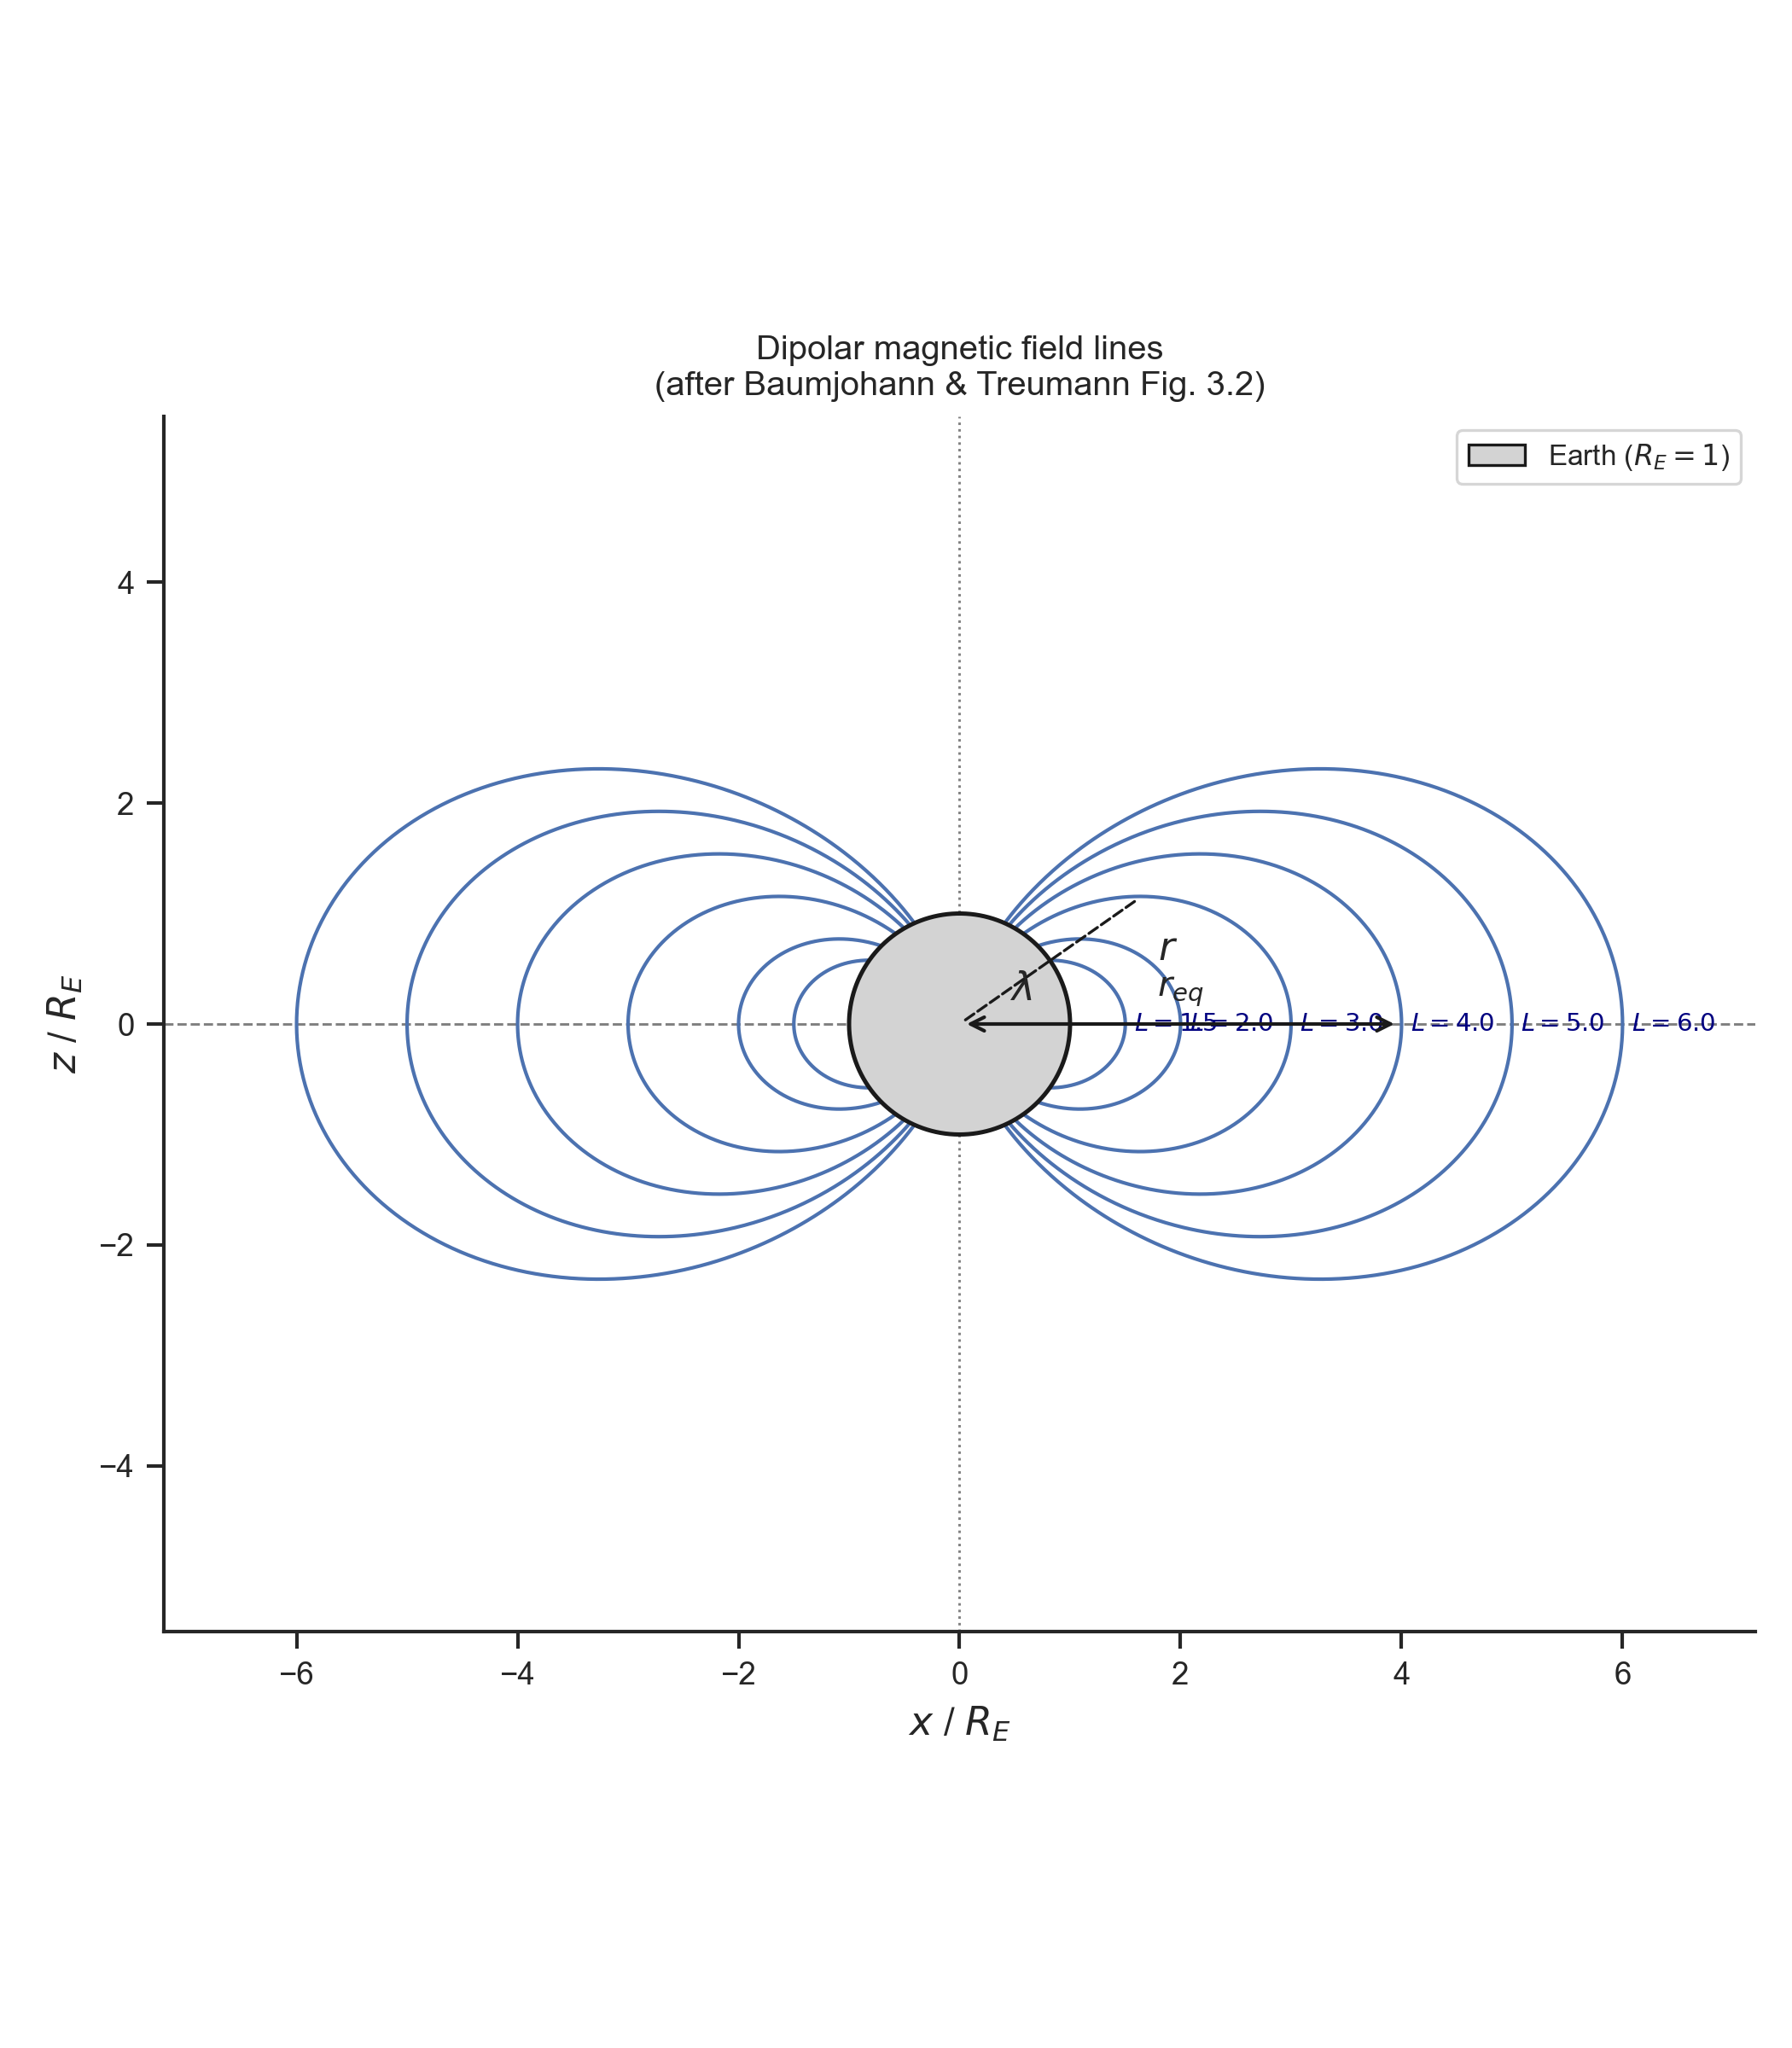
\includegraphics[width=0.6\textwidth]{Figures/test12_dipole_field_lines.png}
  \caption{Dipolar magnetic field lines for $L = 1.5$ to $6$, with Earth
    shown as a filled circle. The equatorial crossing distance $r_\mathrm{eq}
    = L\,R_E$ labels each shell. After Baumjohann \& Treumann
    \citep{baumjohann1996}, Fig.~3.2.}
  \label{fig:field_lines}
\end{figure}

\section{Particle Orbit in the Dipole Field}
\label{sec:dipole_orbit}

A particle is placed at $\mathbf{r}_0 = (3, 0, 0.2)$ in the dipole
field~\eqref{eq:dipole} with $M = 50$ (dimensionless units), speed $v = 1$,
and equatorial pitch angle $\alpha_\mathrm{eq} = 60^\circ$. The trajectory
is integrated for $T = 100$ time units.

With $M = 50$ the gyroradius-to-equatorial-distance ratio is
$\rho/r_\mathrm{eq} \approx 0.16$ and the bounce-to-gyroperiod ratio is
$T_b/T_\Omega \approx 7$. The particle is only marginally adiabatic at
these parameters --- the gyration is visible in the raw orbit, and the
guiding-centre approximation is not expected to be highly accurate. This
choice is deliberate: it makes all three characteristic motions
(gyration, bounce and azimuthal drift) visible simultaneously in the
figures. A well-adiabatic case with $M = 500$ is used in
Sections~\ref{sec:mu}--\ref{sec:gc_vs_full} to test the guiding-centre
theory quantitatively.

Figure~\ref{fig:dipole_bounce} shows the bounce motion. The particle
oscillates between northern and southern mirror points, with
$v_\parallel$ reversing sign at each reflection. The bounce is regular
and the mirror latitudes are consistent across successive cycles.
Figure~\ref{fig:dipole_3D} shows the full 3D orbit: the particle gyrates
around field lines, bounces between hemispheres, and drifts slowly in
longitude.

\begin{figure}[htbp]
  \centering
  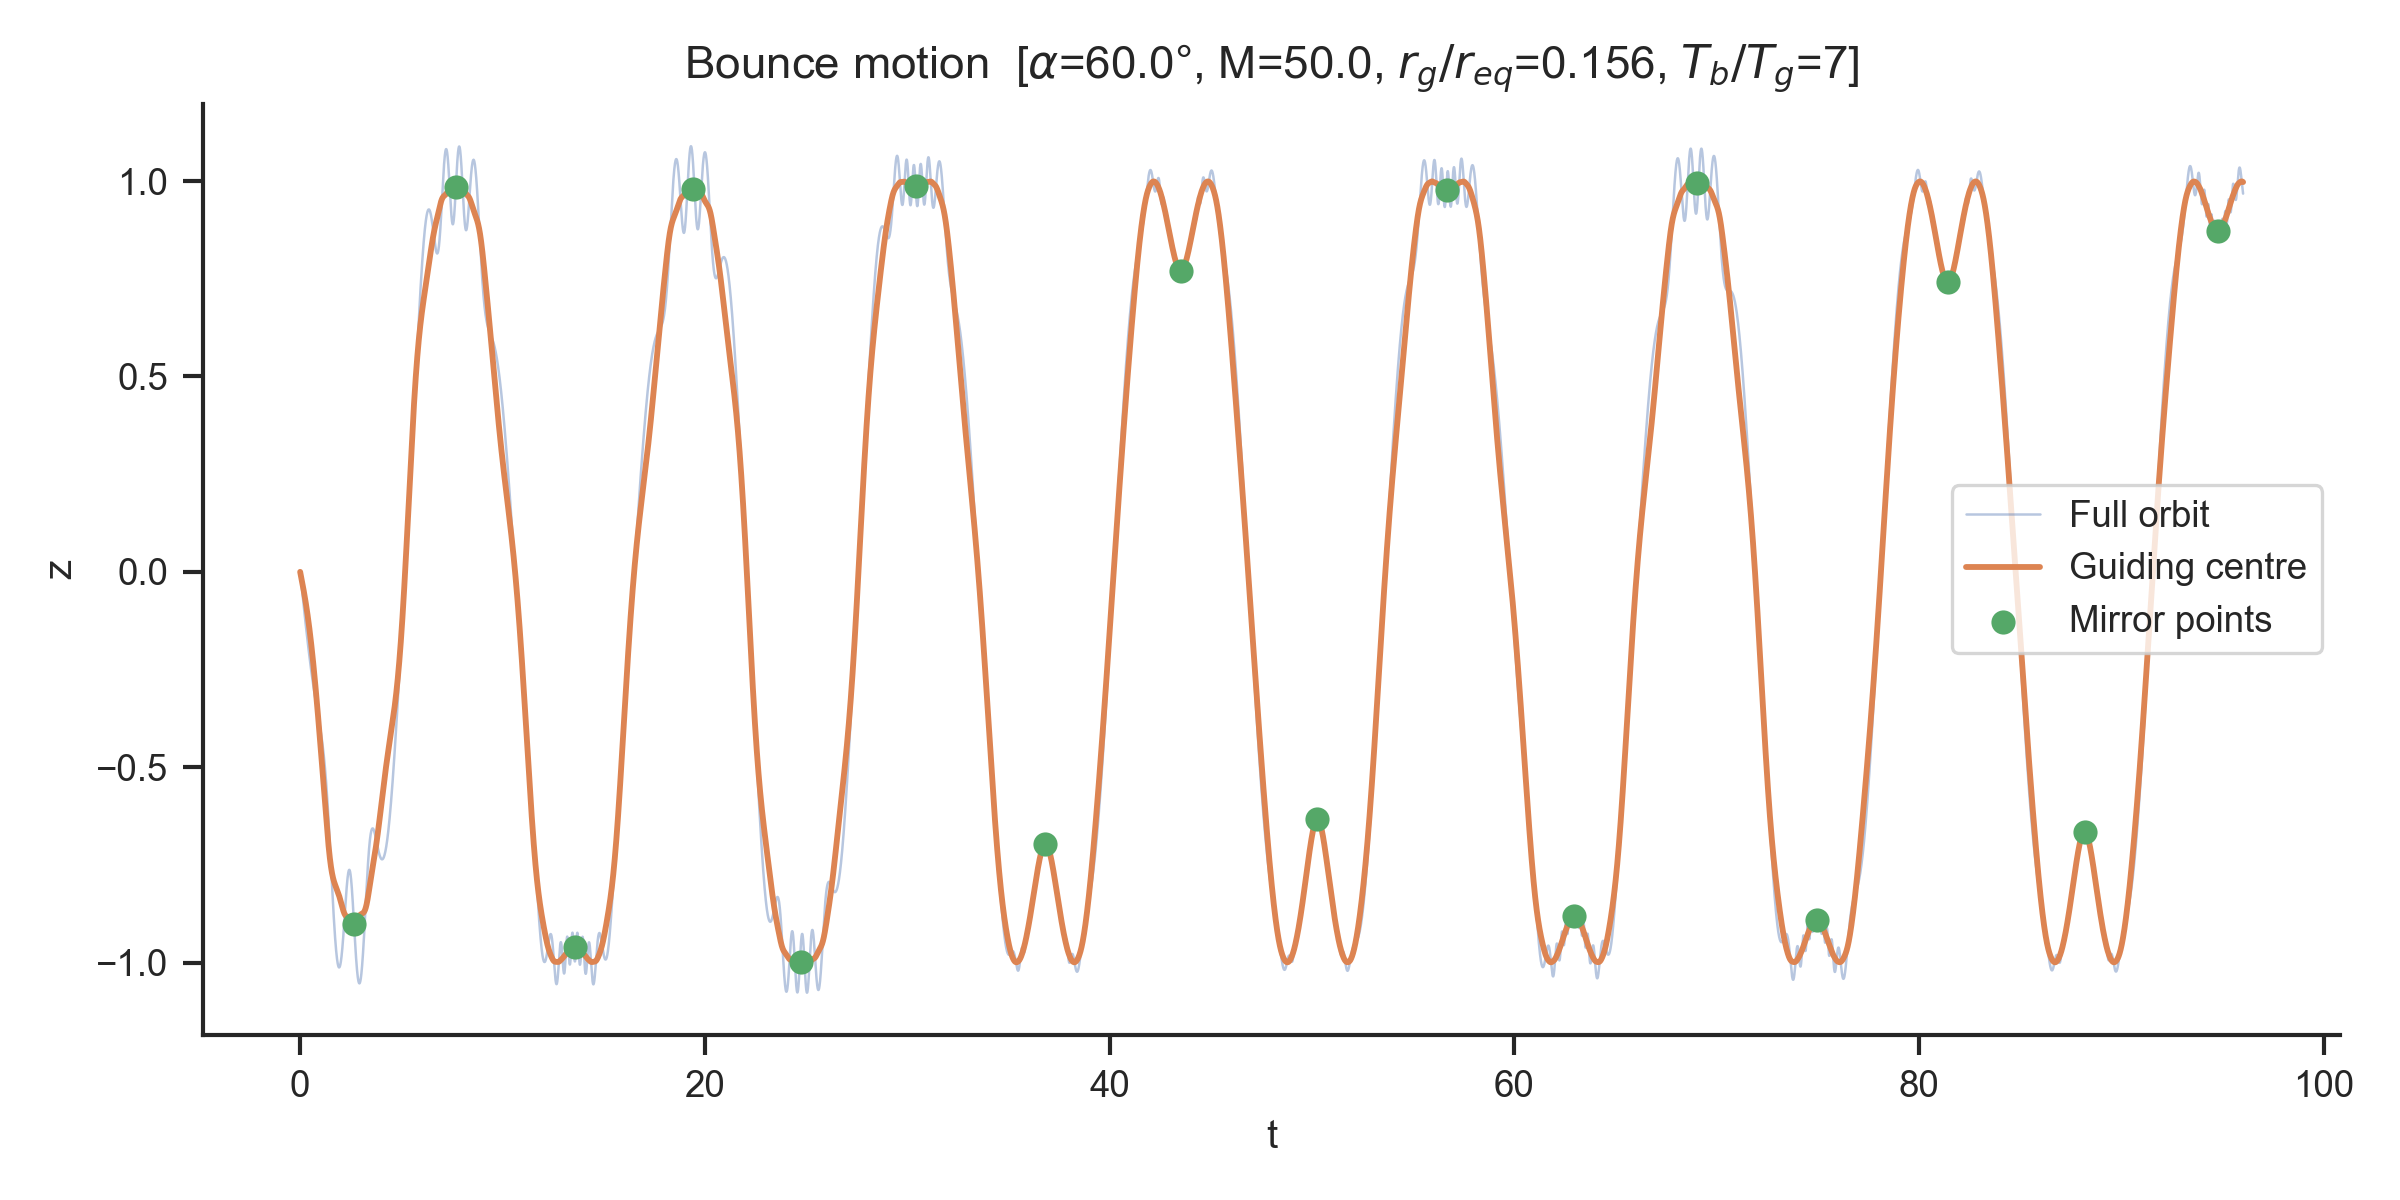
\includegraphics[width=0.65\textwidth]{Figures/test08_dipole_z_vs_t.png}
  \caption{Bounce motion in the dipole field ($M = 50$,
    $\alpha_\mathrm{eq} = 60^\circ$): full orbit (faint) and guiding centre
    (solid), with mirror points marked. The marginally adiabatic parameters
    make the gyration visible in the raw orbit.}
  \label{fig:dipole_bounce}
\end{figure}

\begin{figure}[htbp]
  \centering
  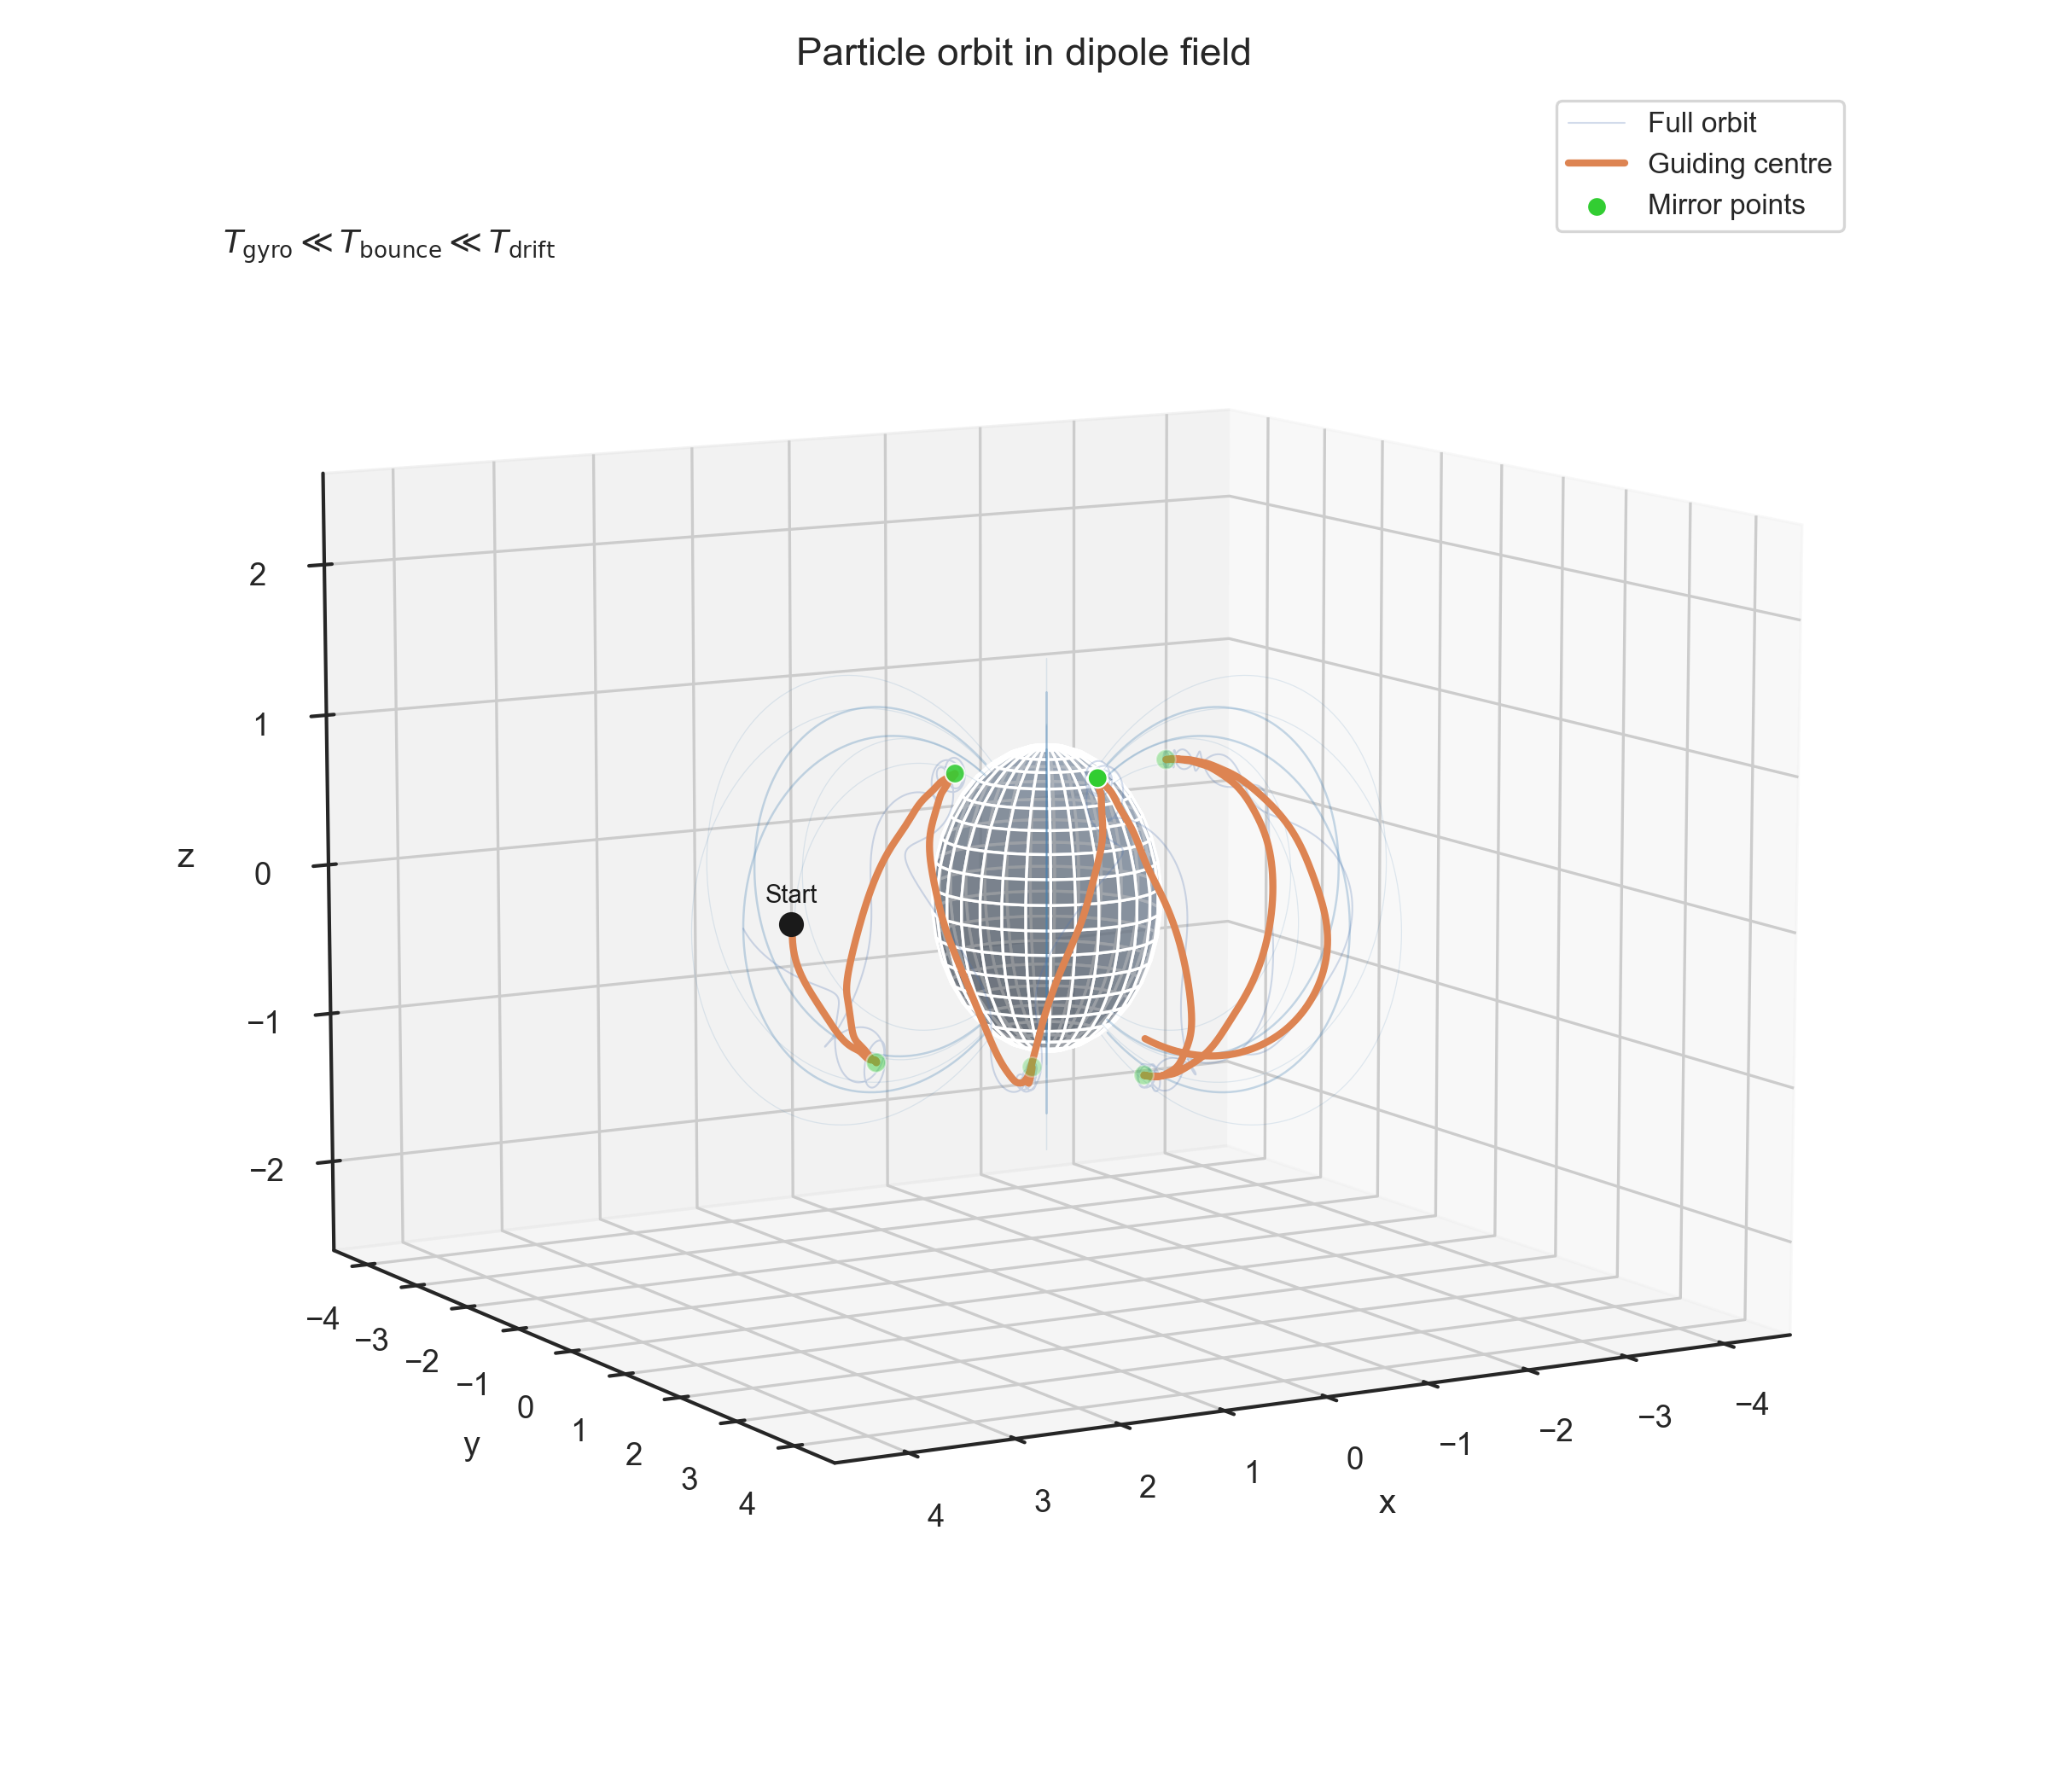
\includegraphics[width=0.55\textwidth]{Figures/test08_dipole_orbit_3D.png}
  \caption{3D orbit in the dipole field, showing gyromotion around field
    lines, bounce between mirror points, and slow azimuthal drift. The
    guiding-centre trajectory (solid) is extracted using
    equation~\eqref{eq:gc_extract}.}
  \label{fig:dipole_3D}
\end{figure}

\section{Magnetic Moment Conservation}
\label{sec:mu}

The magnetic moment $\mu = m v_\perp^2 / 2B$ is an adiabatic invariant:
it is approximately conserved whenever the field varies slowly compared
with the gyration, as expressed by the adiabatic
conditions~\eqref{eq:adiabatic_condition}. Conservation of $\mu$ is what
makes the mirror effect work --- as a particle moves into a region of
stronger $B$, $v_\perp$ must increase to keep $\mu$ constant, and
$v_\parallel$ decreases until the particle is reflected.

To test $\mu$ conservation quantitatively, a stronger dipole ($M = 500$)
is used with $L = 3$ and $\alpha_\mathrm{eq} = 45^\circ$, giving
$\rho/r_\mathrm{eq} \approx 0.006$ and $T_b/T_\Omega \approx 100$ ---
well into the adiabatic regime. Figure~\ref{fig:mu} shows the relative
variation $|\delta\mu/\mu_0|$ over four bounce periods.

\begin{figure}[htbp]
  \centering
  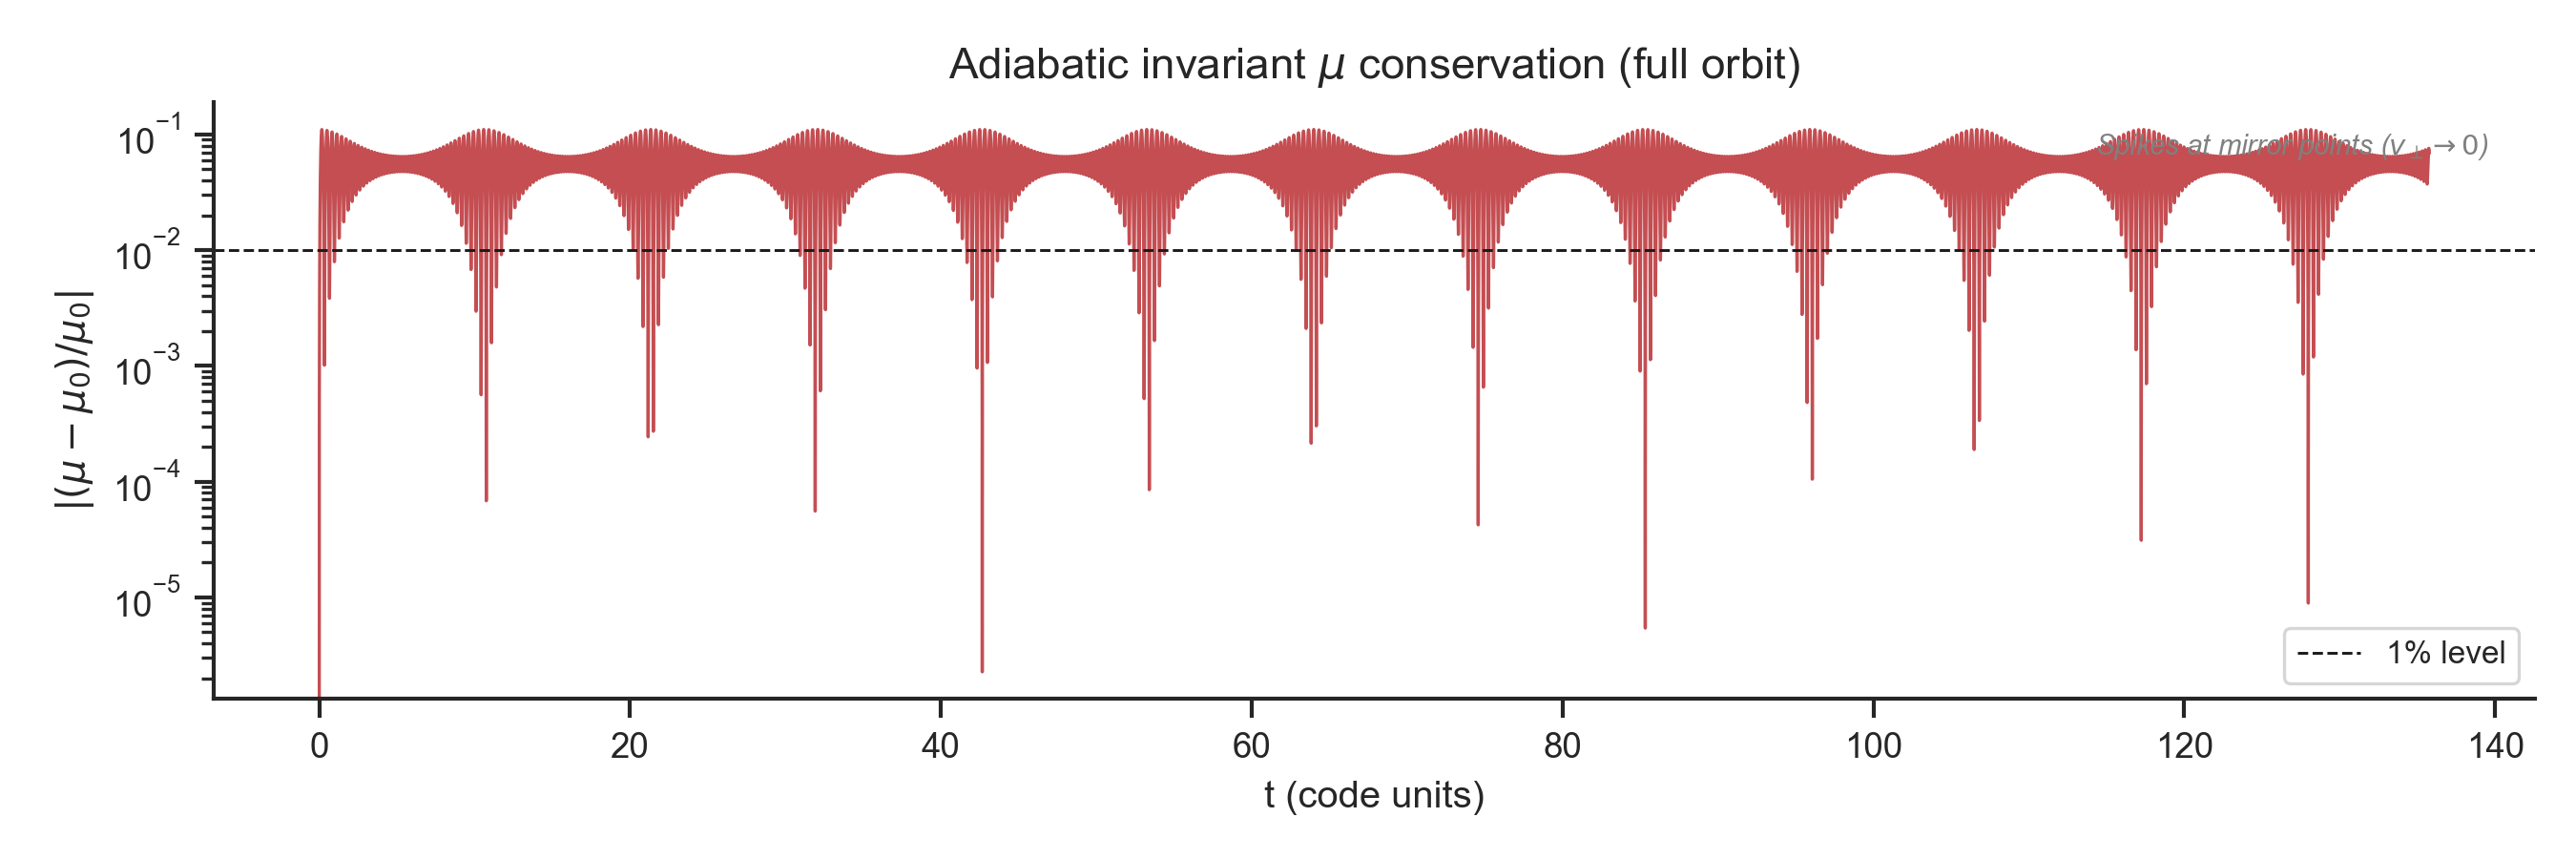
\includegraphics[width=0.7\textwidth]{Figures/test11_mu_conservation.png}
  \caption{Relative variation of $\mu$ over four bounce periods
    ($M = 500$, $L = 3$, $\alpha_\mathrm{eq} = 45^\circ$). The periodic
    spikes occur at mirror points, where $v_\perp \to 0$ makes the ratio
    $\mu/\mu_0$ numerically sensitive. Between mirror points, $\mu$ is
    conserved to well below 1\,\% (dashed line).}
  \label{fig:mu}
\end{figure}

Between mirror points the variation stays well below the 1\,\% level,
confirming that the adiabatic condition is comfortably satisfied for
these parameters. The periodic spikes coincide with mirror points, where
$v_\perp \to 0$ and $B$ is large; the ratio $\delta\mu/\mu_0$ becomes
numerically sensitive at these instants but returns to a small value
immediately afterwards. This is a feature of the diagnostic, not a
failure of conservation.

\section{Guiding-Centre Approximation versus Full Orbit}
\label{sec:gc_vs_full}

The guiding-centre (GC) approximation replaces the fast gyromotion with
a smooth drift trajectory, valid when $\rho \ll L$ and
$T_\Omega \ll T_b$. To test this, three representations of the same
motion are computed simultaneously in the dipole field with $M = 500$,
$L = 3$, $\alpha_\mathrm{eq} = 45^\circ$:
\begin{enumerate}
  \item the full Lorentz orbit,
  \item the guiding-centre position extracted from that orbit using
    equation~\eqref{eq:gc_extract},
  \item an independent solution of the GC equations of
    motion~\eqref{eq:gc_r}--\eqref{eq:gc_vpar}, started from the same
    initial guiding-centre position.
\end{enumerate}

For these parameters the gyroradius is $\rho \approx 0.019$ code units,
giving $\rho/r_\mathrm{eq} \approx 0.006 \ll 1$ and
$T_b/T_\Omega \approx 100 \gg 1$. Both adiabatic conditions are
comfortably satisfied.

Figure~\ref{fig:gc_z} overlays $z(t)$ from all three solutions over four
bounce periods. The extracted GC and the GC equations solution track each
other closely, with no visible phase drift in the bounce envelope. The
positional separation between the extracted GC and the GC equations
solution stays well below one gyroradius throughout the integration.

\begin{figure}[htbp]
  \centering
  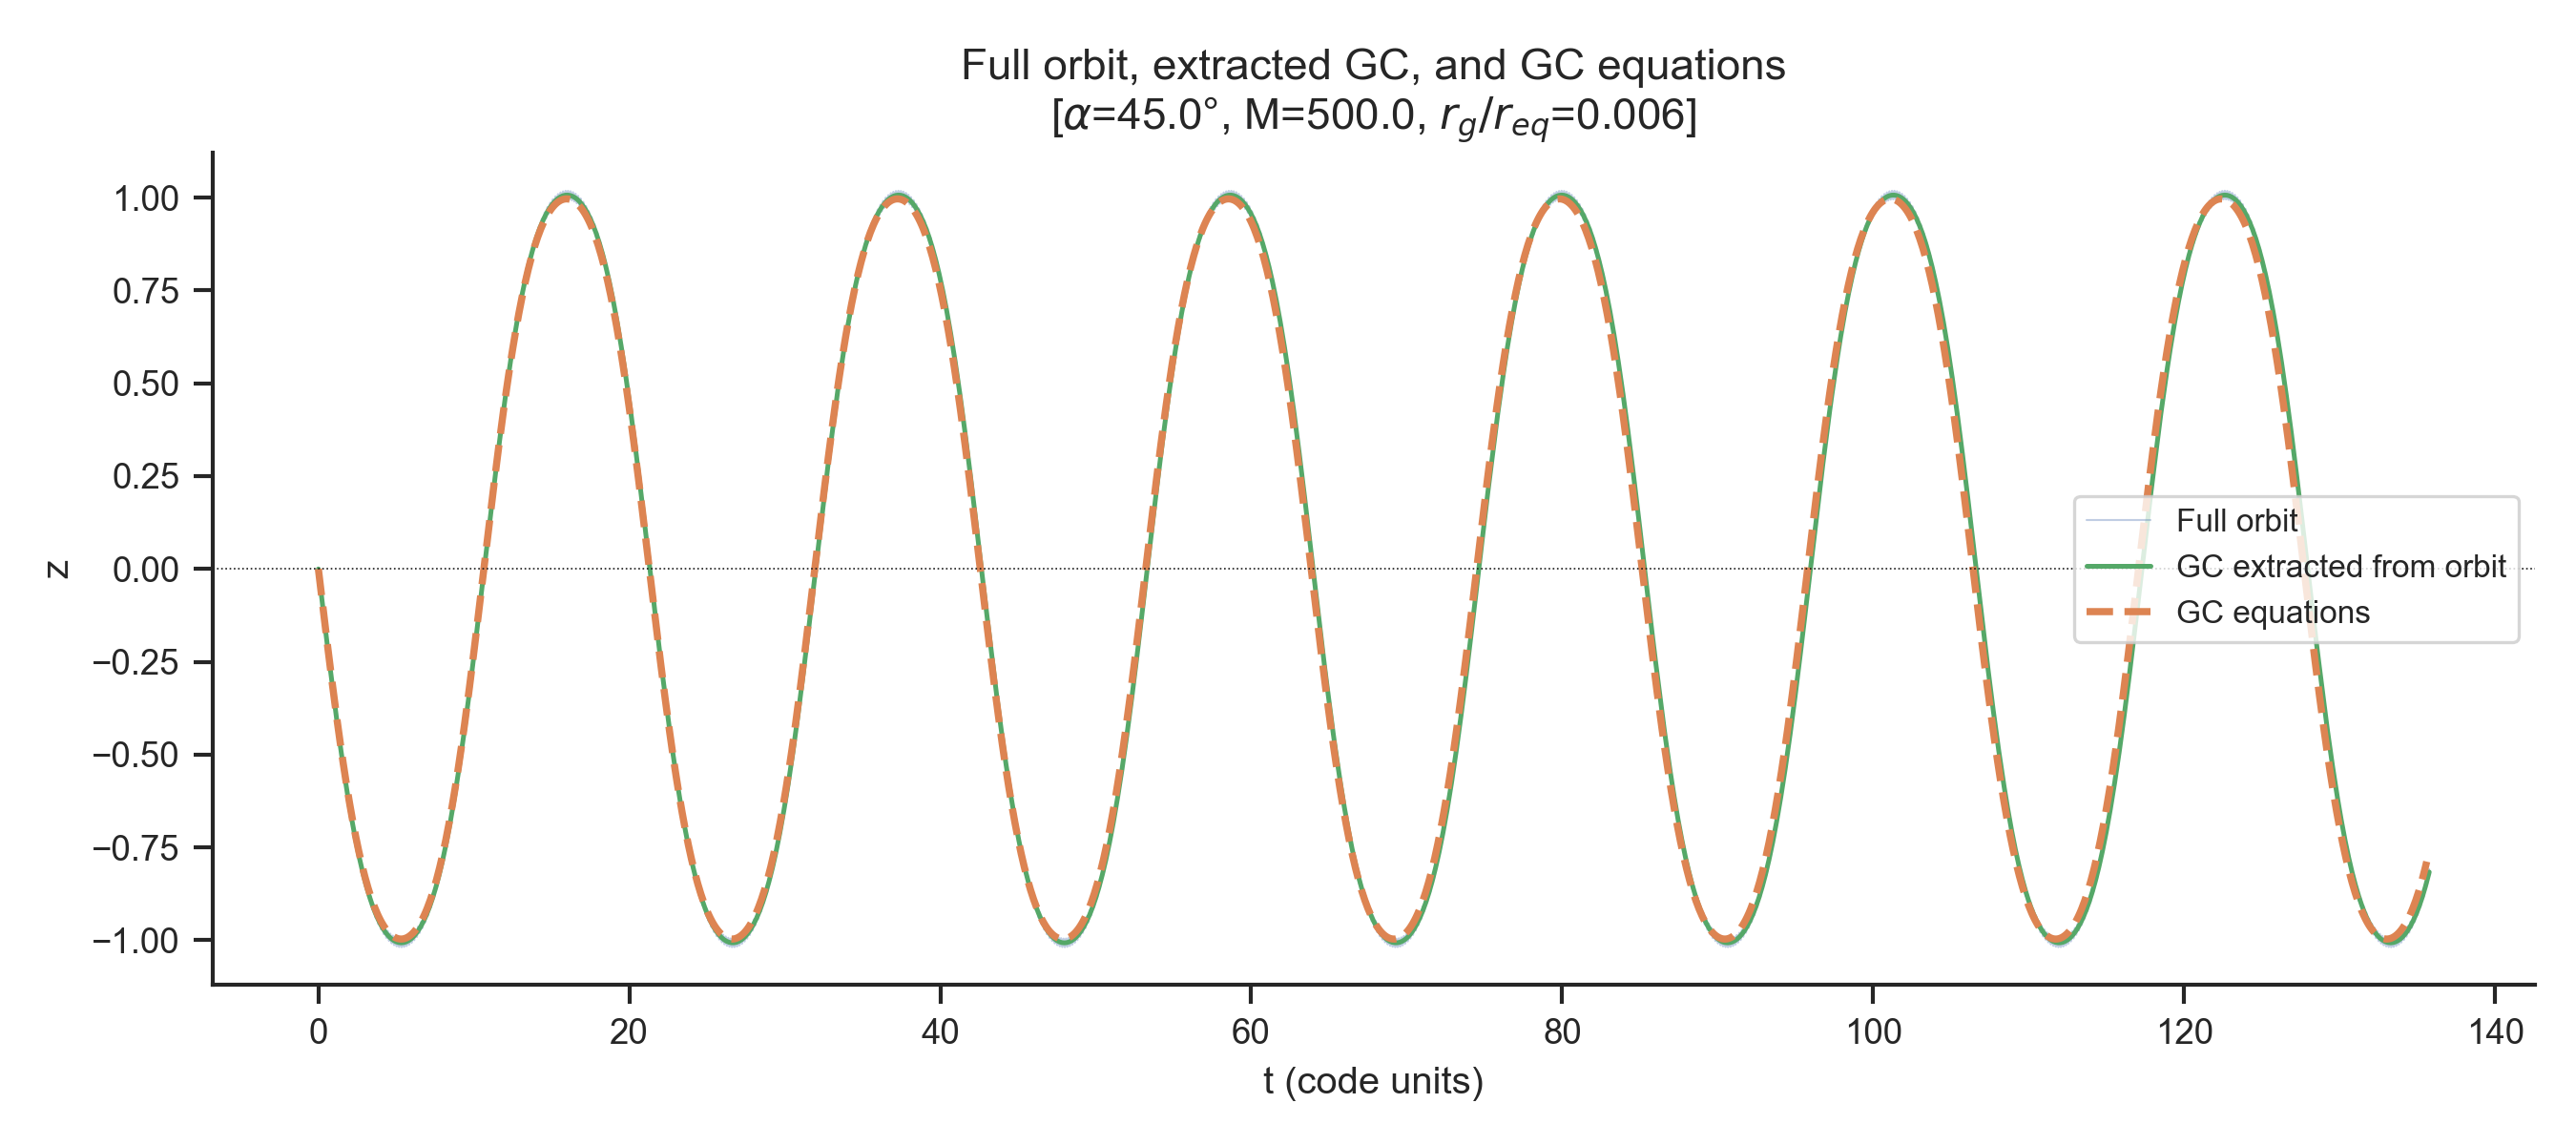
\includegraphics[width=0.65\textwidth]{Figures/test11_gc_vs_full_z.png}
  \caption{Full orbit vs guiding-centre approximation ($M = 500$,
    $L = 3$, $\alpha_\mathrm{eq} = 45^\circ$): $z(t)$ from the full
    orbit, the extracted GC, and the GC equations of motion. All three
    overlap on this scale, confirming the validity of the GC
    approximation in the adiabatic regime.}
  \label{fig:gc_z}
\end{figure}

The slow growth of the separation envelope is a consequence of secular
phase drift from the non-symplectic RK45 integrator, not a breakdown of
the adiabatic approximation. Energy conservation of the full Lorentz
orbit remains below $|\delta K| < 10^{-6}$ throughout, and $\mu$ shows
no secular trend (Figure~\ref{fig:mu}).

\section{\texorpdfstring{Physical Units: 10\,keV Electron at $L = 3$}{Physical Units: 10 keV Electron at L=3}}
\label{sec:si_units}

To connect the dimensionless simulations to a physical scenario, a
10\,keV electron is placed at $L = 3$ ($r_\mathrm{eq} = 3R_E$) in
Earth's dipole field with $\alpha_\mathrm{eq} = 45^\circ$. The dipole
moment is $M_E = 8.05 \times 10^{22}$\,A\,m$^2$
\citep{baumjohann1996}, and the equatorial field strength at this
$L$-shell is $B_\mathrm{eq} = B_E/L^3 \approx 1.15\,\mu$T, where
$B_E = 3.11 \times 10^{-5}$\,T.

At this energy and field strength the gyroperiod is
$T_\Omega \approx 32\,\mu$s, the gyroradius is $\rho \approx 0.2$\,km
($3 \times 10^{-5}\,R_E$), and the bounce period is
$\tau_b \approx 1.8$\,s. The ratio
$\rho/r_\mathrm{eq} \approx 10^{-5}$ places the particle deep in the
adiabatic regime, with $T_b/T_\Omega \approx 57{,}000$.

Figure~\ref{fig:si_z} shows $z(t)$ in units of $R_E$ over two bounce
periods. The numerical mirror latitude agrees with the analytic prediction
$\lambda_m = 23.1^\circ$ (from equation~\eqref{eq:mirror} with
$\sin^2\alpha_\mathrm{eq} = 1/2$) to within 0.02\,\%.

\begin{figure}[htbp]
  \centering
  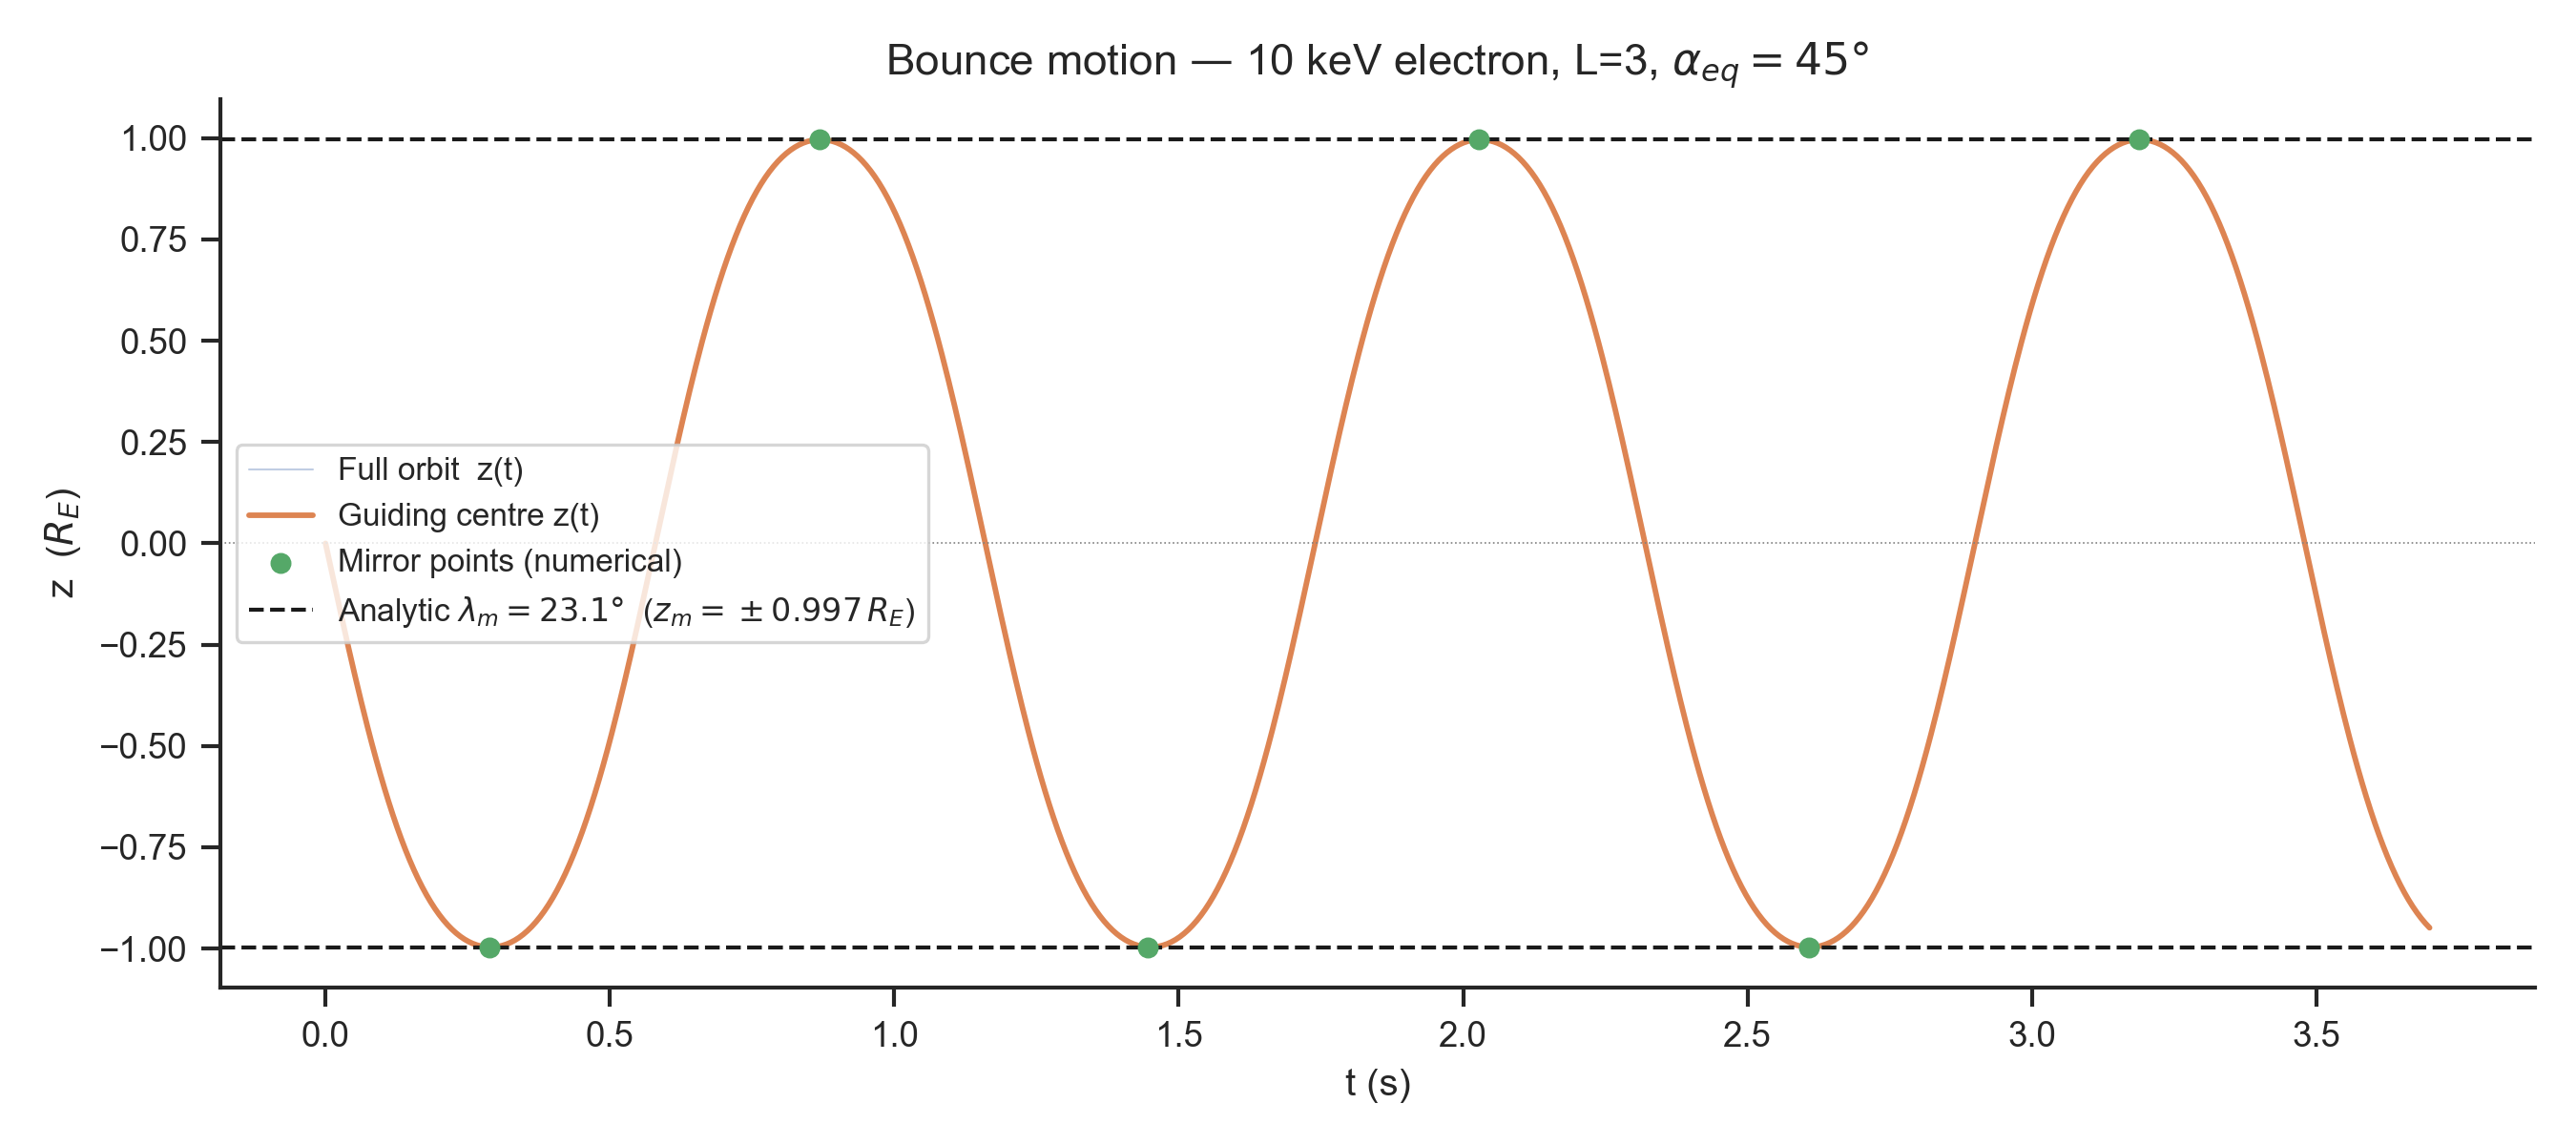
\includegraphics[width=0.6\textwidth]{Figures/test13_SI_z_vs_t.png}
  \caption{Bounce motion of a 10\,keV electron at $L = 3$ in SI units.
    Full orbit (faint), guiding centre (solid), and mirror points (dots).
    The analytic mirror latitude $\lambda_m = 23.1^\circ$ is marked
    (dashed). Agreement is within 0.02\,\%.}
  \label{fig:si_z}
\end{figure}

Over two bounce periods the solver integrates approximately 115{,}000
gyrations. The relative energy drift reaches
$|\delta K| \approx 1.5\,\%$ and $\mu$ varies by approximately 2\,\%
by the end of the run. Both are consistent with secular phase drift from
the non-symplectic integrator over this many cycles; the physically
meaningful check is the mirror point accuracy, which remains excellent.
A symplectic integrator (such as the Boris method) would improve
long-term phase tracking for runs of this length.

\section{Tilted Dipole}
\label{sec:tilted}

In most planetary magnetospheres the magnetic dipole axis is not aligned
with the rotation axis. For Earth the tilt is only $11^\circ$, but for
Neptune it is approximately $47^\circ$ and for Uranus approximately
$59^\circ$ \citep{baumjohann1996}. A tilted dipole produces asymmetric
bounce motion when viewed in geographic coordinates, because the
magnetic equatorial plane no longer coincides with the geographic
equatorial plane.

The tilted dipole field is obtained by rotating the dipole moment vector
away from the $z$-axis by a tilt angle $\theta_\mathrm{tilt}$ in the
$x$--$z$ plane, so that
$\hat{\mathbf{m}} = (\sin\theta_\mathrm{tilt}, 0,
\cos\theta_\mathrm{tilt})$. The field
expression~\eqref{eq:dipole} generalises straightforwardly by replacing
$\hat{\mathbf{z}}$ with $\hat{\mathbf{m}}$. Three runs are performed
with $M = 500$, $L = 3$, $\alpha_\mathrm{eq} = 45^\circ$, and tilt
angles of $0^\circ$, $47^\circ$ and $59^\circ$. Each particle is
initialised on its magnetic equatorial plane so that the initial
conditions are equivalent across all three cases in magnetic coordinates.

Figure~\ref{fig:tilt_z} compares $z(t)$ in geographic coordinates. At
$0^\circ$ the bounce is symmetric about $z = 0$. At $47^\circ$ and
$59^\circ$ the bounce midpoint shifts to negative $z$ (the magnetic
equator sits below the geographic equator), and the amplitudes in the
two hemispheres become unequal. The particle still mirrors correctly in
all cases: the bounce period and mirror latitudes in magnetic coordinates
are unchanged, and the asymmetry is purely a coordinate effect.

\begin{figure}[htbp]
  \centering
  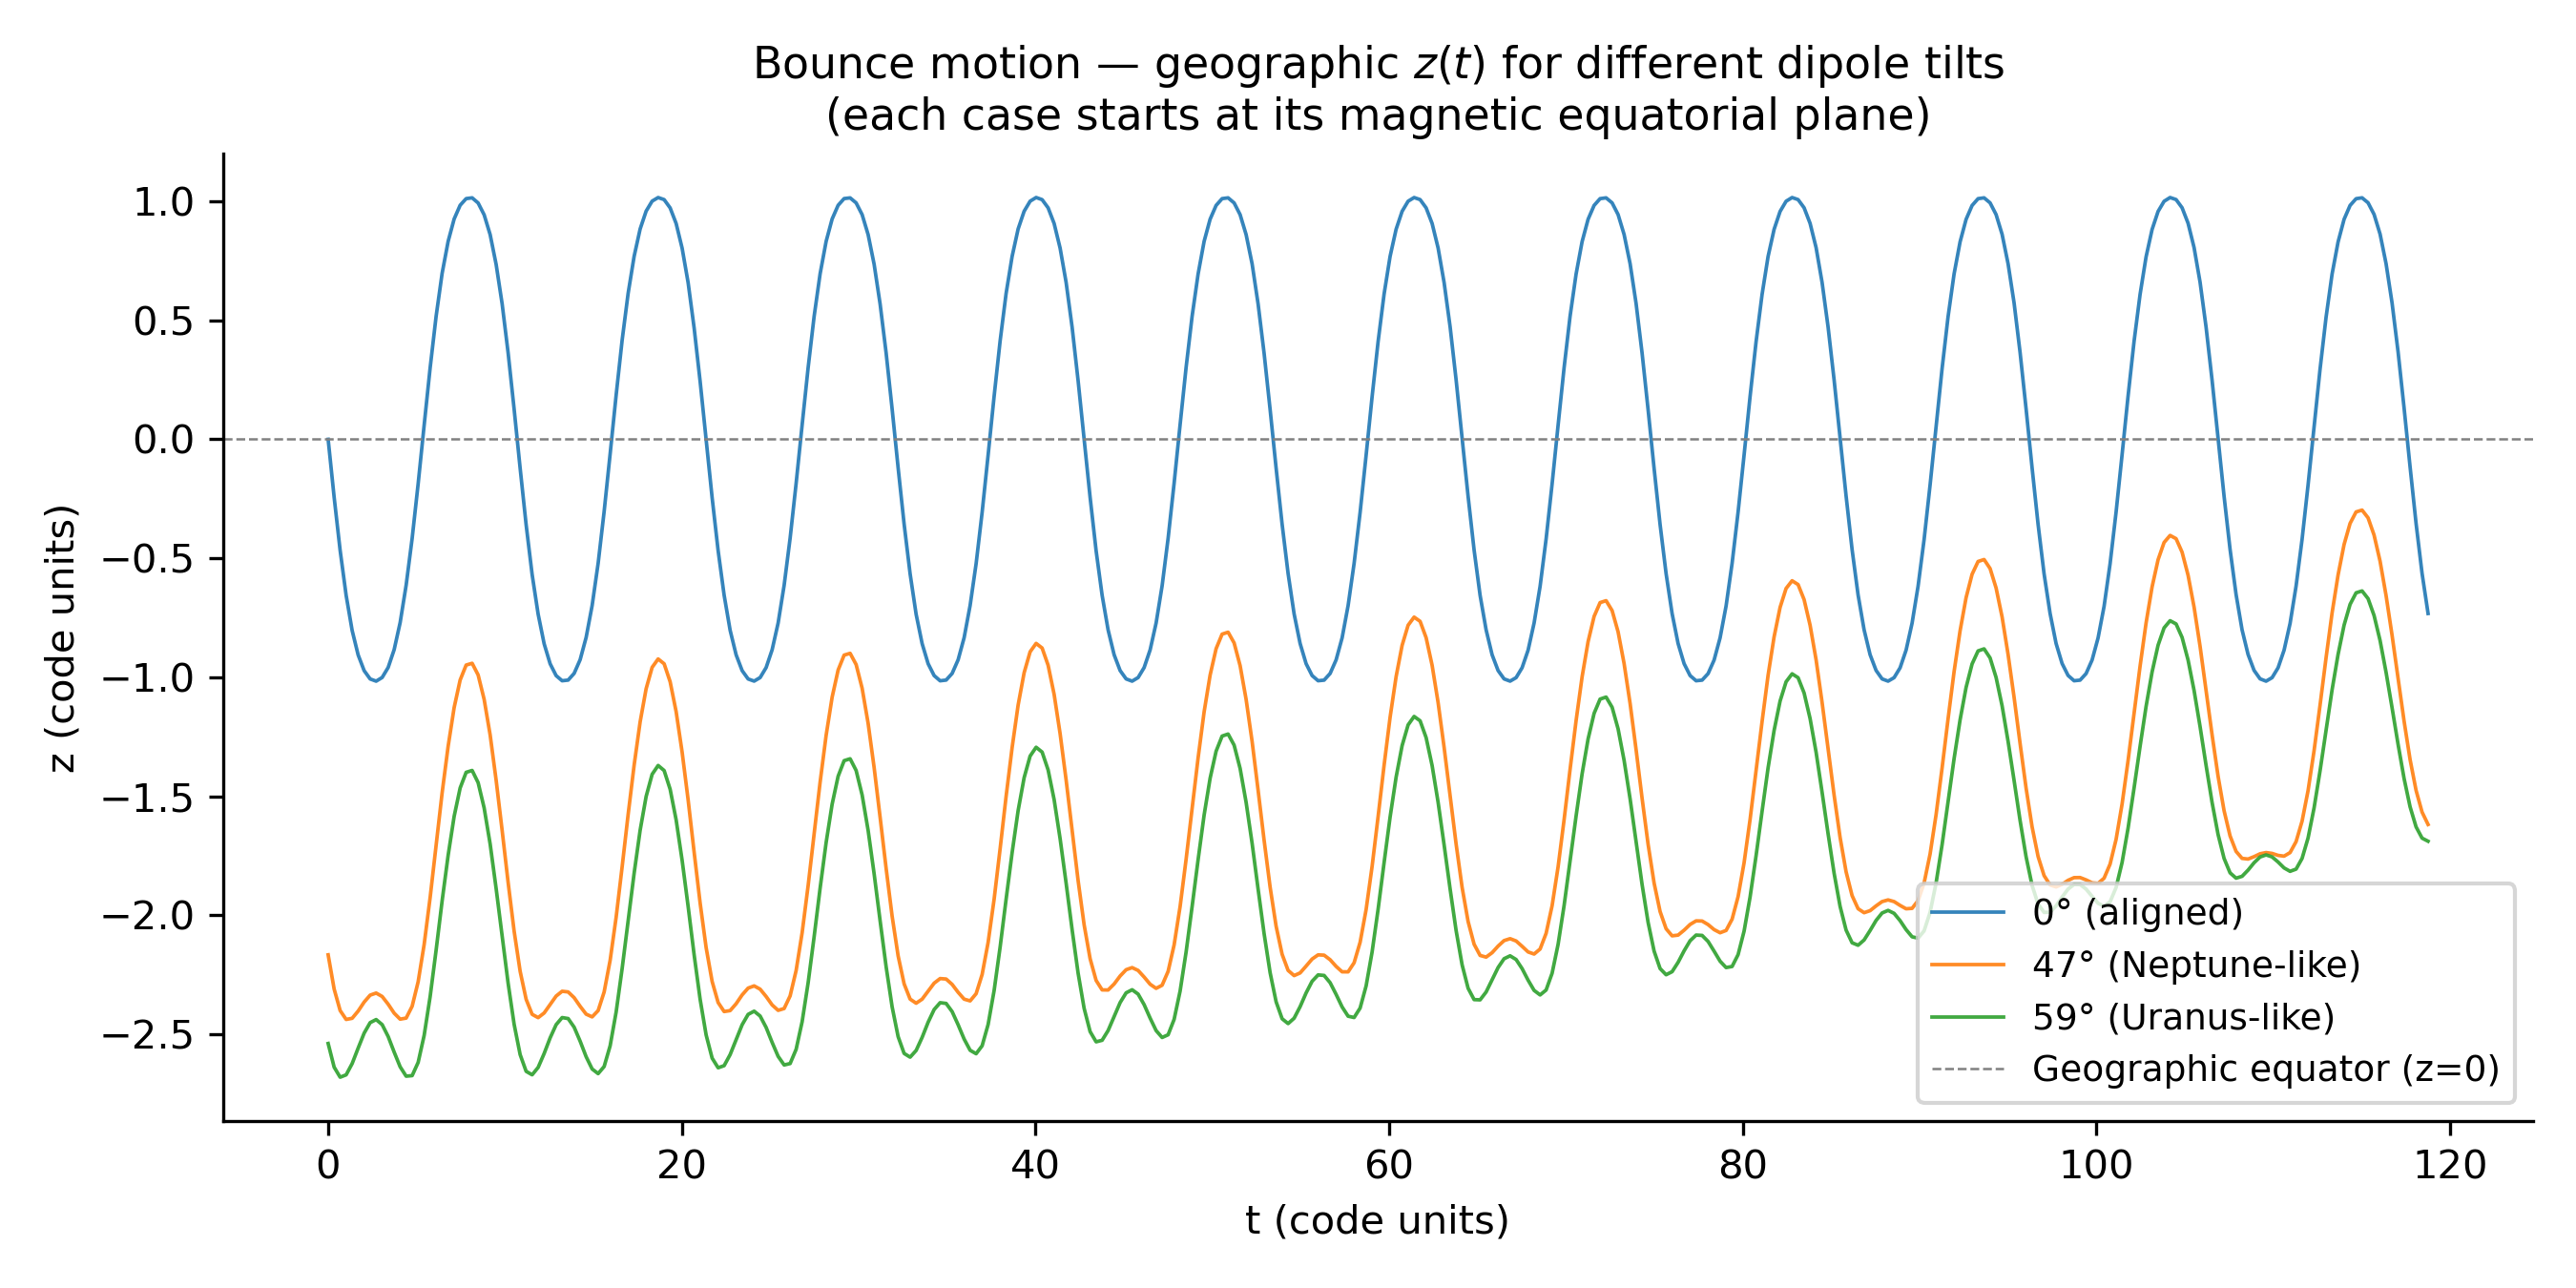
\includegraphics[width=0.65\textwidth]{Figures/test14_z_vs_t_tilt_comparison.png}
  \caption{Geographic $z(t)$ for tilt angles $0^\circ$, $47^\circ$
    (Neptune-like) and $59^\circ$ (Uranus-like). Bounce becomes
    increasingly asymmetric as the magnetic equator tilts away from
    the geographic equatorial plane.}
  \label{fig:tilt_z}
\end{figure}

Figure~\ref{fig:tilt_3D} shows the 3D guiding-centre trajectory for the
$59^\circ$ case (Uranus-like). The drift shell is visibly tilted relative to the
geographic equatorial plane, and the particle traces out a path that
follows the tilted dipole field lines.

\begin{figure}[htbp]
  \centering
  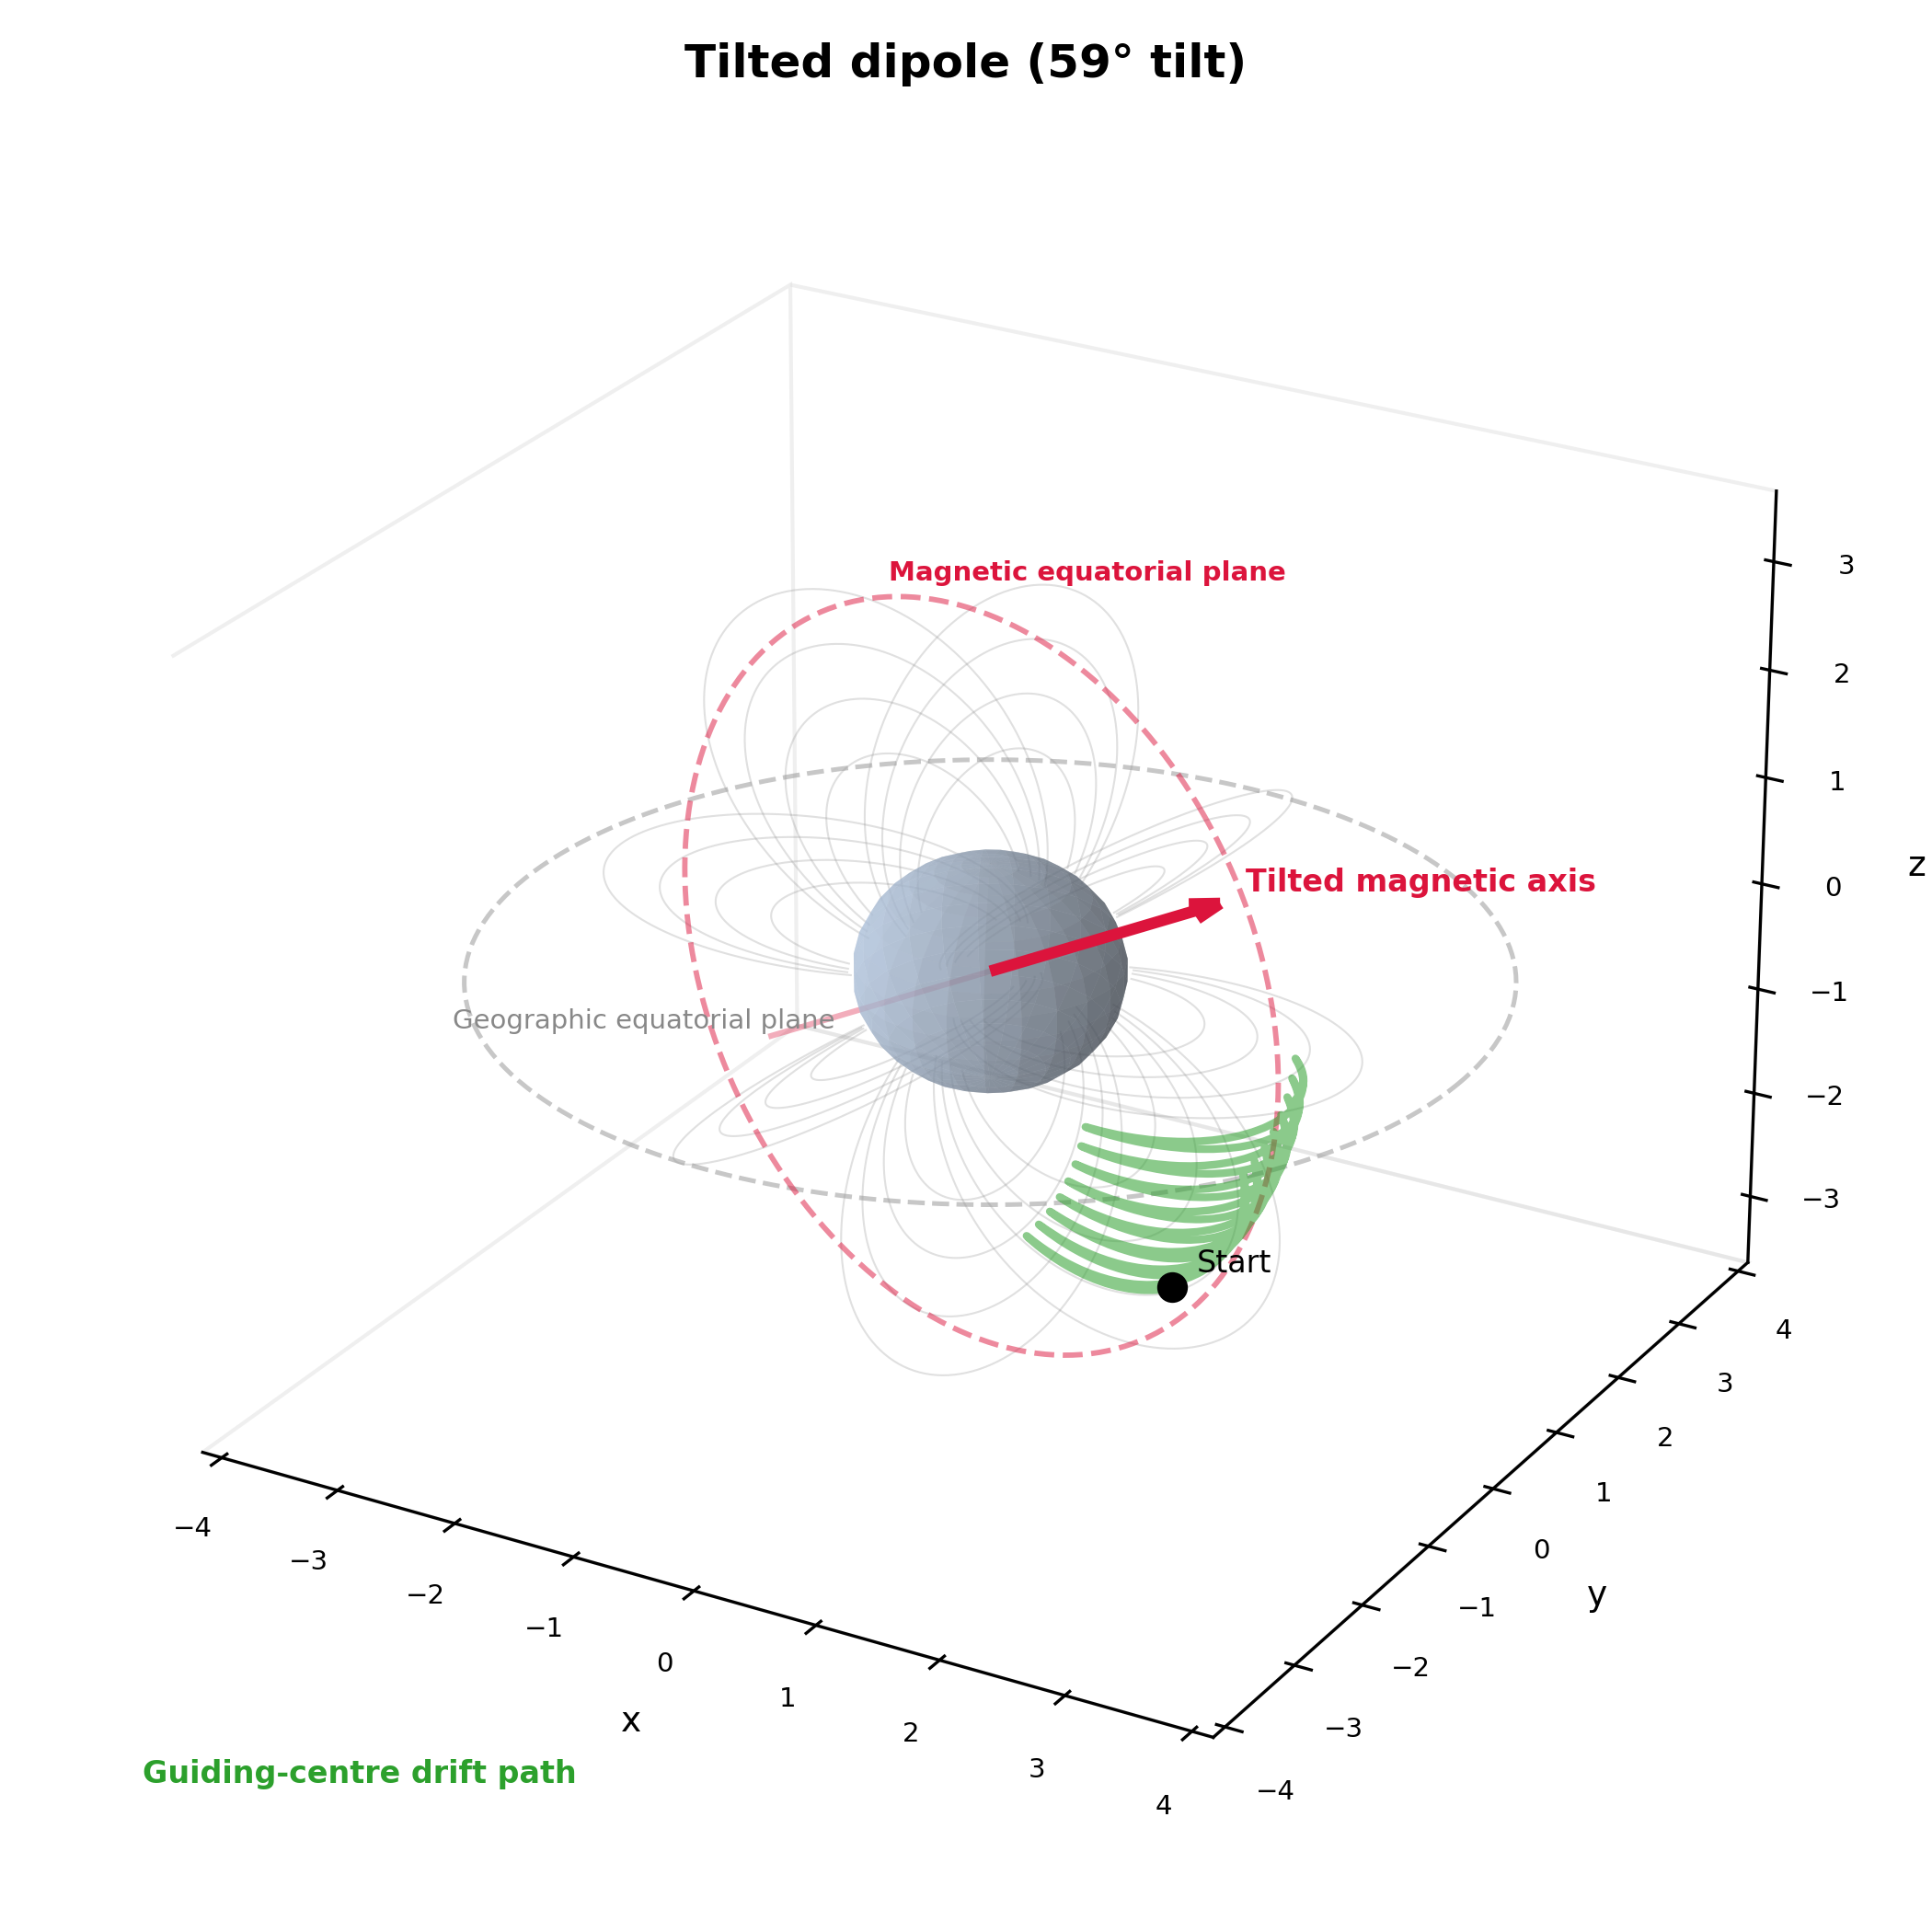
\includegraphics[width=0.55\textwidth]{Figures/test14_orbit_3D_tilted.png}
  \caption{3D guiding-centre orbit in a $59^\circ$-tilted dipole field
    (Uranus-like). The magnetic axis (red) is tilted from the geographic
    equatorial plane (grey dashed). The GC drift path (green) follows
    the tilted field geometry.}
  \label{fig:tilt_3D}
\end{figure}

\section{Corotation}
\label{sec:corotation}

In a planetary magnetosphere, the corotation electric field
$\mathbf{E} = -(\boldsymbol{\Omega} \times \mathbf{r}) \times \mathbf{B}$
drives an $\mathbf{E} \times \mathbf{B}$ drift that locks the plasma to
the planet's rotation at angular velocity $\Omega$. However, gradient
and curvature drifts are always present on top of this, so the total
azimuthal drift rate exceeds $\Omega$ slightly:
\[
  \Omega_\mathrm{total} = \Omega_{E \times B} + \Omega_{\nabla B}
    + \Omega_\mathrm{curv} \;>\; \Omega.
\]

To isolate the $\mathbf{E} \times \mathbf{B}$ contribution, two runs
are made with identical initial conditions ($M = 500$, $L = 3$,
$\alpha_\mathrm{eq} = 45^\circ$, $\Omega = 0.02$): one with the
corotation electric field and one without.

Figure~\ref{fig:corotation} shows the guiding-centre trajectory under
corotation, coloured by time. The total azimuthal drift rate is
$\Omega_\mathrm{total} \approx 0.027$. Subtracting the gradient and
curvature drift contribution ($\Omega_{\nabla B + c} \approx 0.008$,
measured from a separate run without the electric field) gives an
$\mathbf{E} \times \mathbf{B}$ contribution of $0.019$, recovering the
input $\Omega = 0.020$ to within 96.6\,\%. This confirms that the
corotation electric field is implemented correctly.

\begin{figure}[htbp]
  \centering
  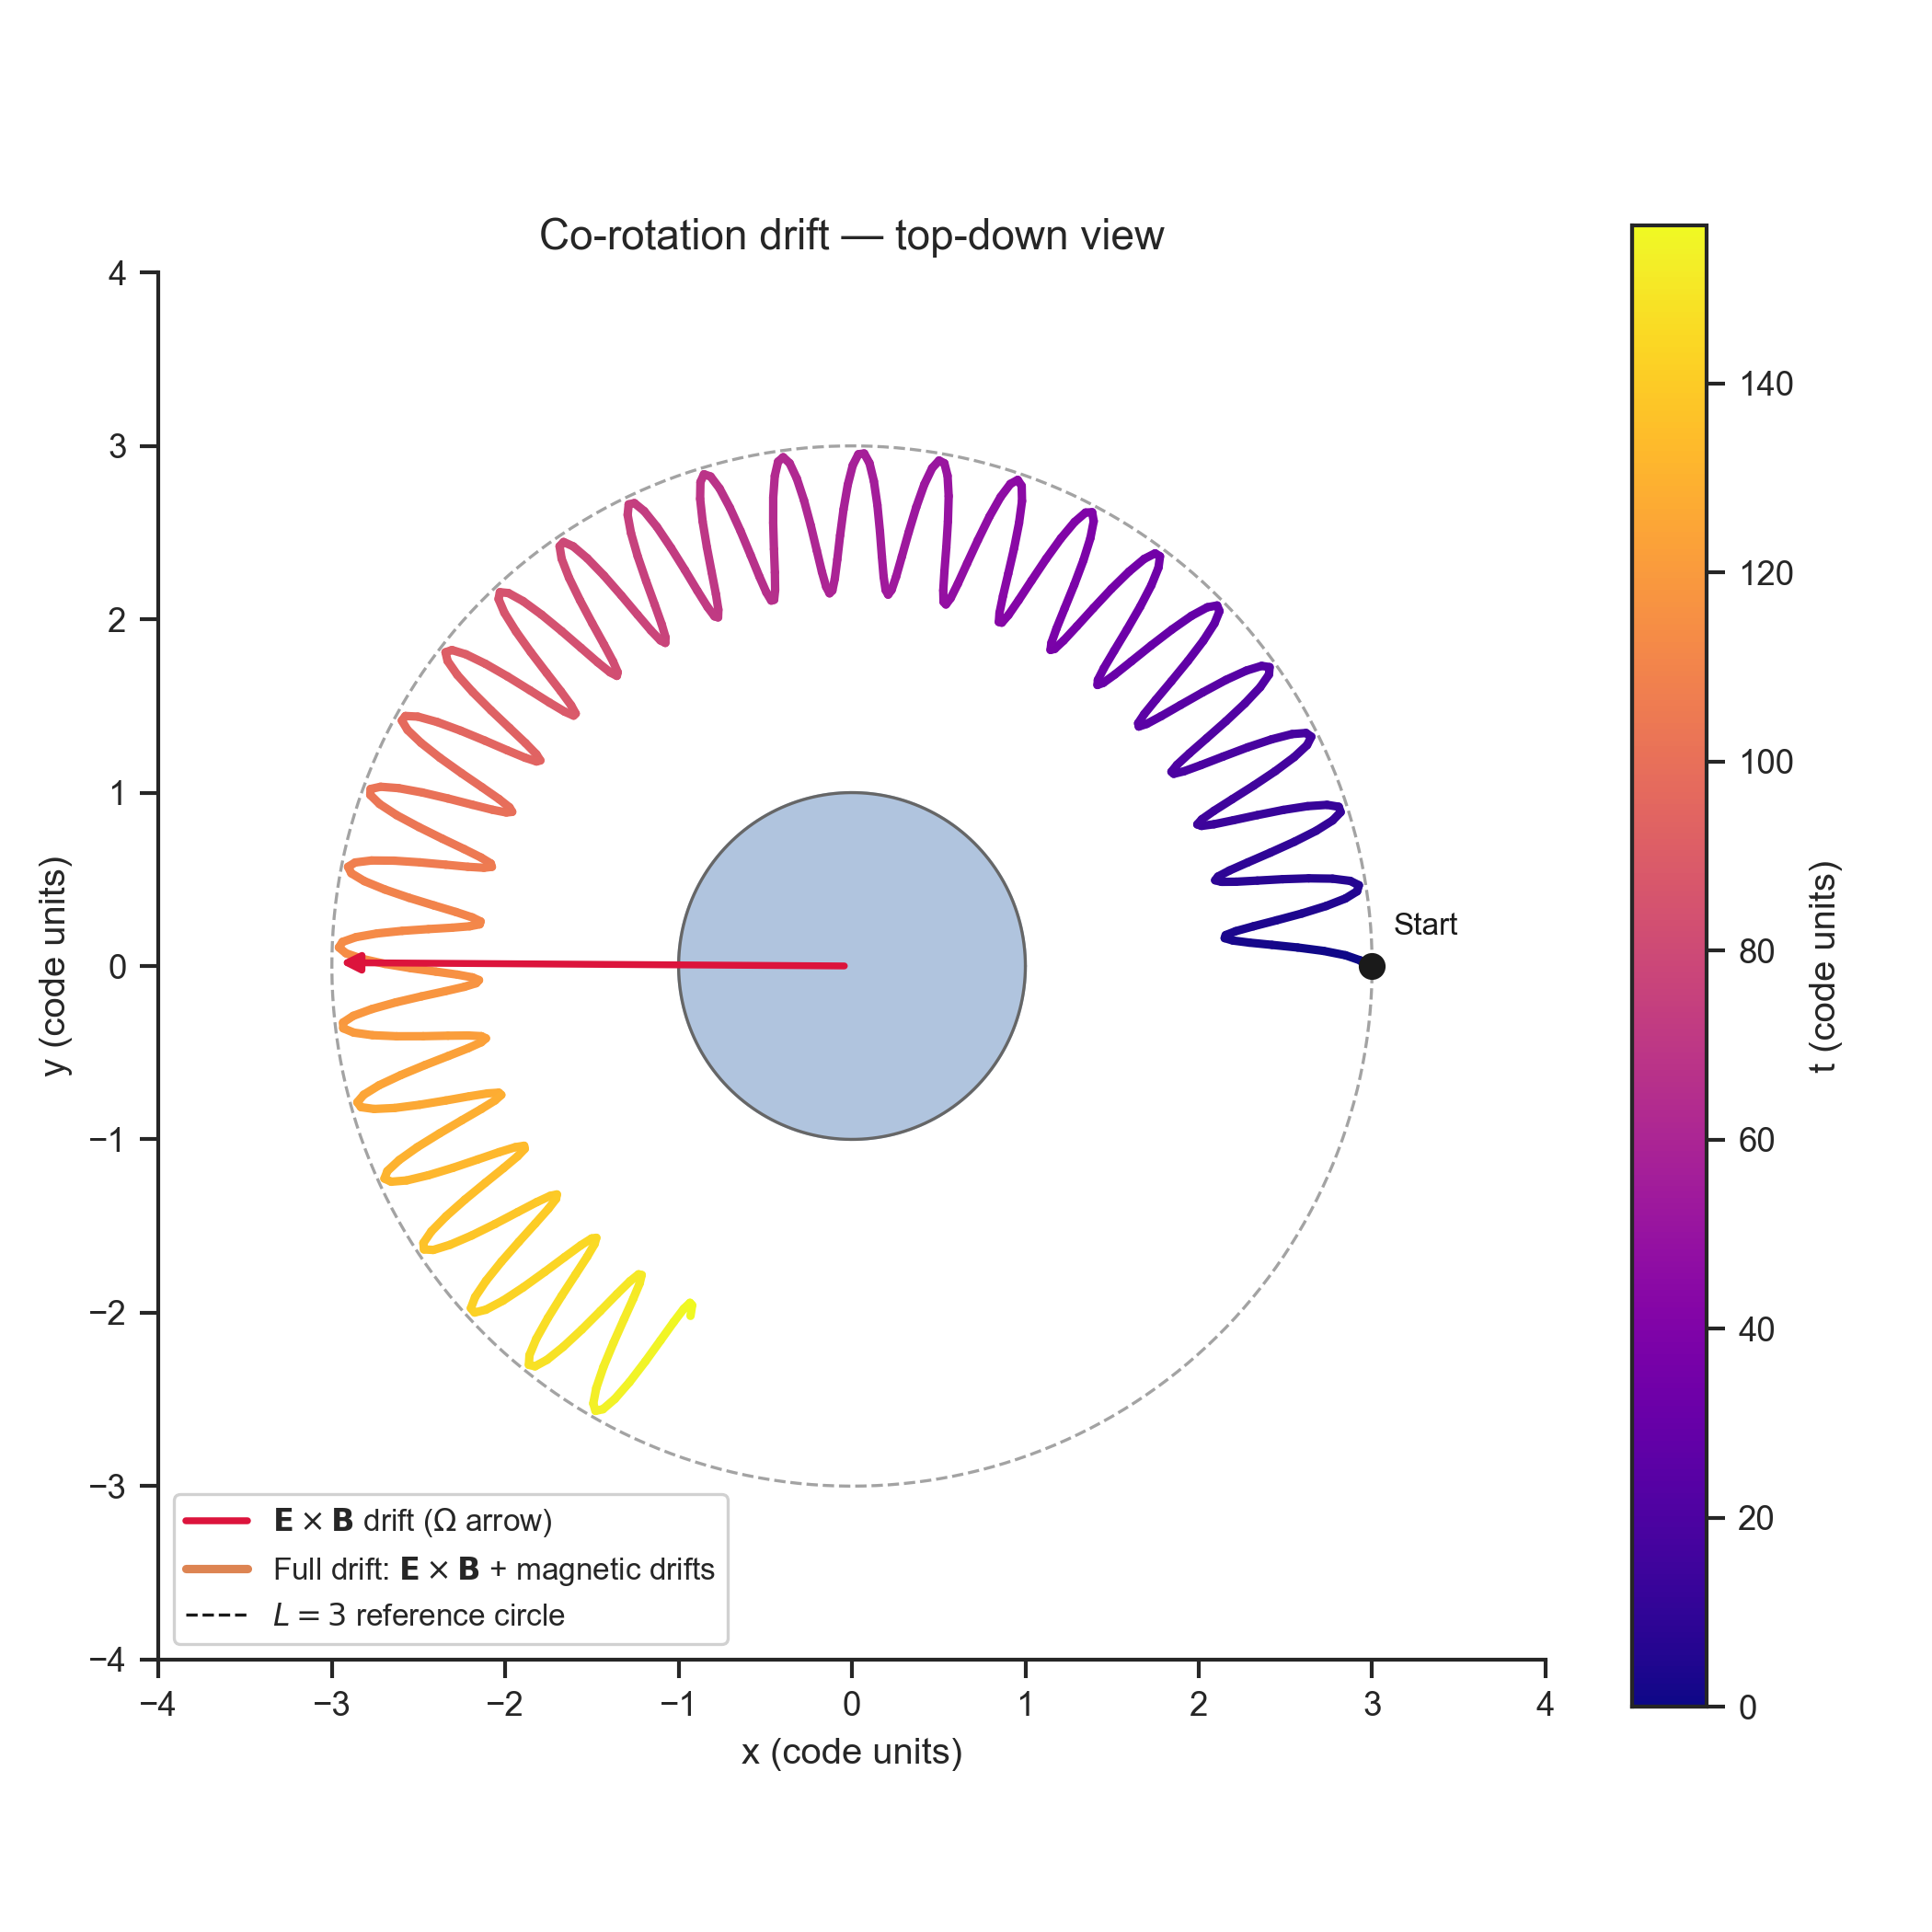
\includegraphics[width=0.6\textwidth]{Figures/test15_corotation_xy.png}
  \caption{Top-down view of the guiding-centre trajectory under corotation
    ($\Omega = 0.02$), coloured by time. The GC drifts azimuthally near
    the $L = 3$ reference circle (dashed). The crimson arrow shows the
    planet's rotation over the same interval.}
  \label{fig:corotation}
\end{figure}

The small shortfall of $\sim\!3.4\,\%$ in the recovery is physical, not
numerical: the corotation electric field has a small component along
$\mathbf{B}$ in the equatorial region that slightly reduces the
effective perpendicular drift. Bounce motion persists throughout, with
the same mirror latitudes as in the $\mathbf{E} = \mathbf{0}$ case.

\section{Rotating Tilted Dipole}
\label{sec:rotating}

The most realistic simulation combines all three ingredients: a tilted
dipole axis ($\theta_\mathrm{tilt} = 47^\circ$, Neptune-like), planetary
rotation at $\Omega = 0.02$, and the corotation electric field
$\mathbf{E} = -(\boldsymbol{\Omega} \times \mathbf{r}) \times
\mathbf{B}(\mathbf{r}, t)$. The dipole moment now rotates about the
$z$-axis, making the magnetic field time-dependent. The integrator
evaluates $\mathbf{B}(\mathbf{r}, t)$ at each timestep.

The particle is initialised on the magnetic equatorial plane at $L = 3$
with $\alpha_\mathrm{eq} = 45^\circ$ and integrated for one full
rotation period $T_\mathrm{rot} = 2\pi/\Omega \approx 314$ code time
units. All three adiabatic timescales are well separated:
$T_\Omega \approx 0.34$, $T_b \approx 17$, $T_\mathrm{rot} \approx 314$.

Figure~\ref{fig:rot_z} shows $z(t)$. The bounce amplitude is modulated
by the rotating field geometry: as the tilted dipole sweeps past the
particle, the local field configuration changes, and the mirror latitudes
shift accordingly.

\begin{figure}[htbp]
  \centering
  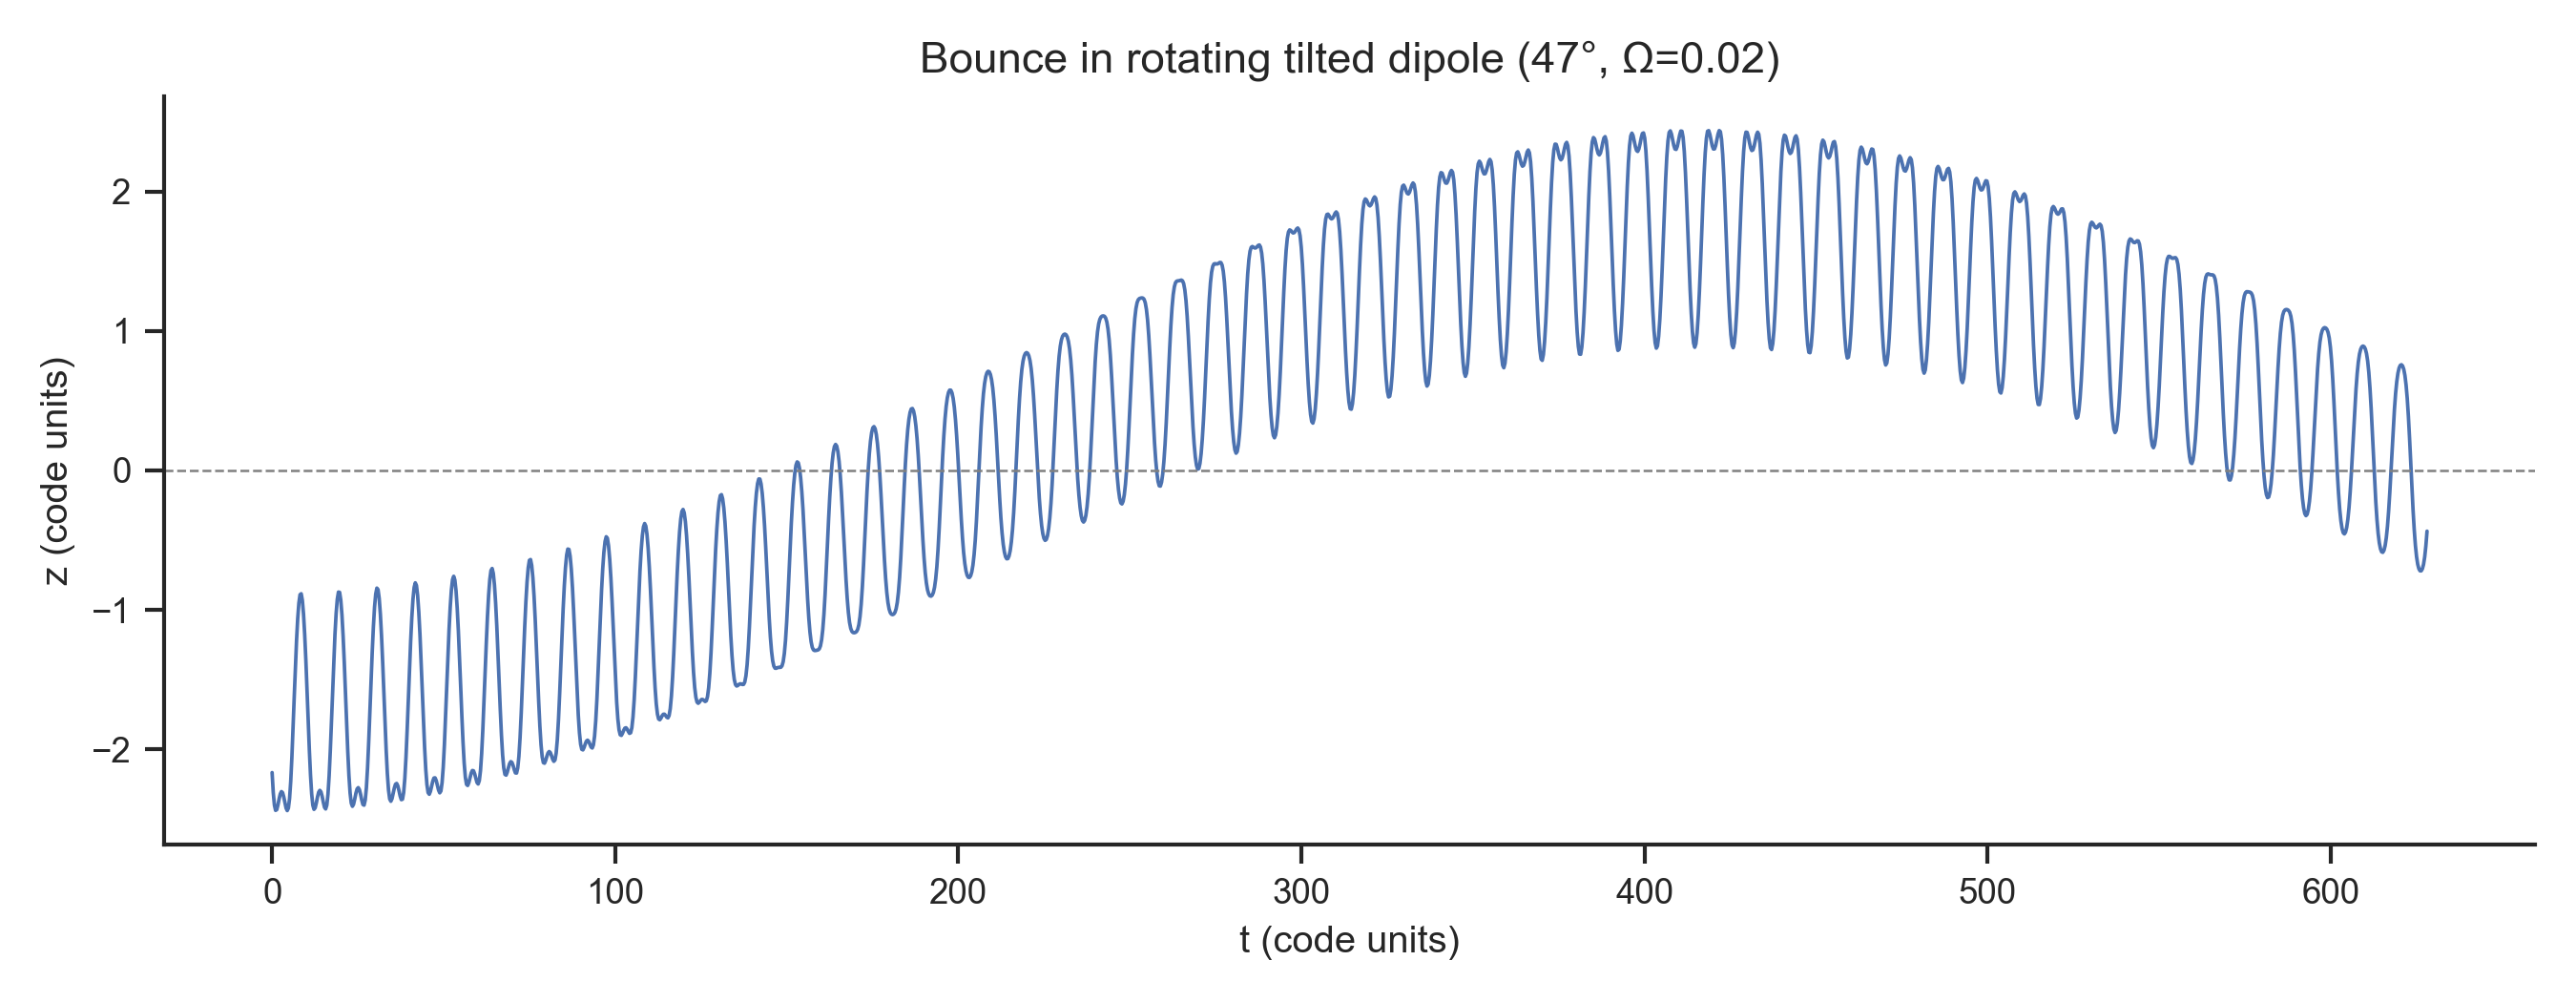
\includegraphics[width=0.7\textwidth]{Figures/test16_rotating_dipole_z_vs_t.png}
  \caption{$z(t)$ in the rotating tilted dipole ($47^\circ$ tilt,
    $\Omega = 0.02$). The bounce amplitude modulates as the tilted
    dipole rotates past the particle.}
  \label{fig:rot_z}
\end{figure}

Figure~\ref{fig:rot_3D} shows the full 3D guiding-centre orbit. The
particle sweeps around the rotation axis while bouncing along the
tilted field lines, tracing out a drift shell that is itself tilted
relative to the geographic equator. This is the most complete simulation
in the project, combining gyration, bounce, gradient and curvature
drifts, $\mathbf{E} \times \mathbf{B}$ corotation, and the
time-dependent field from a rotating tilted dipole.

\begin{figure}[htbp]
  \centering
  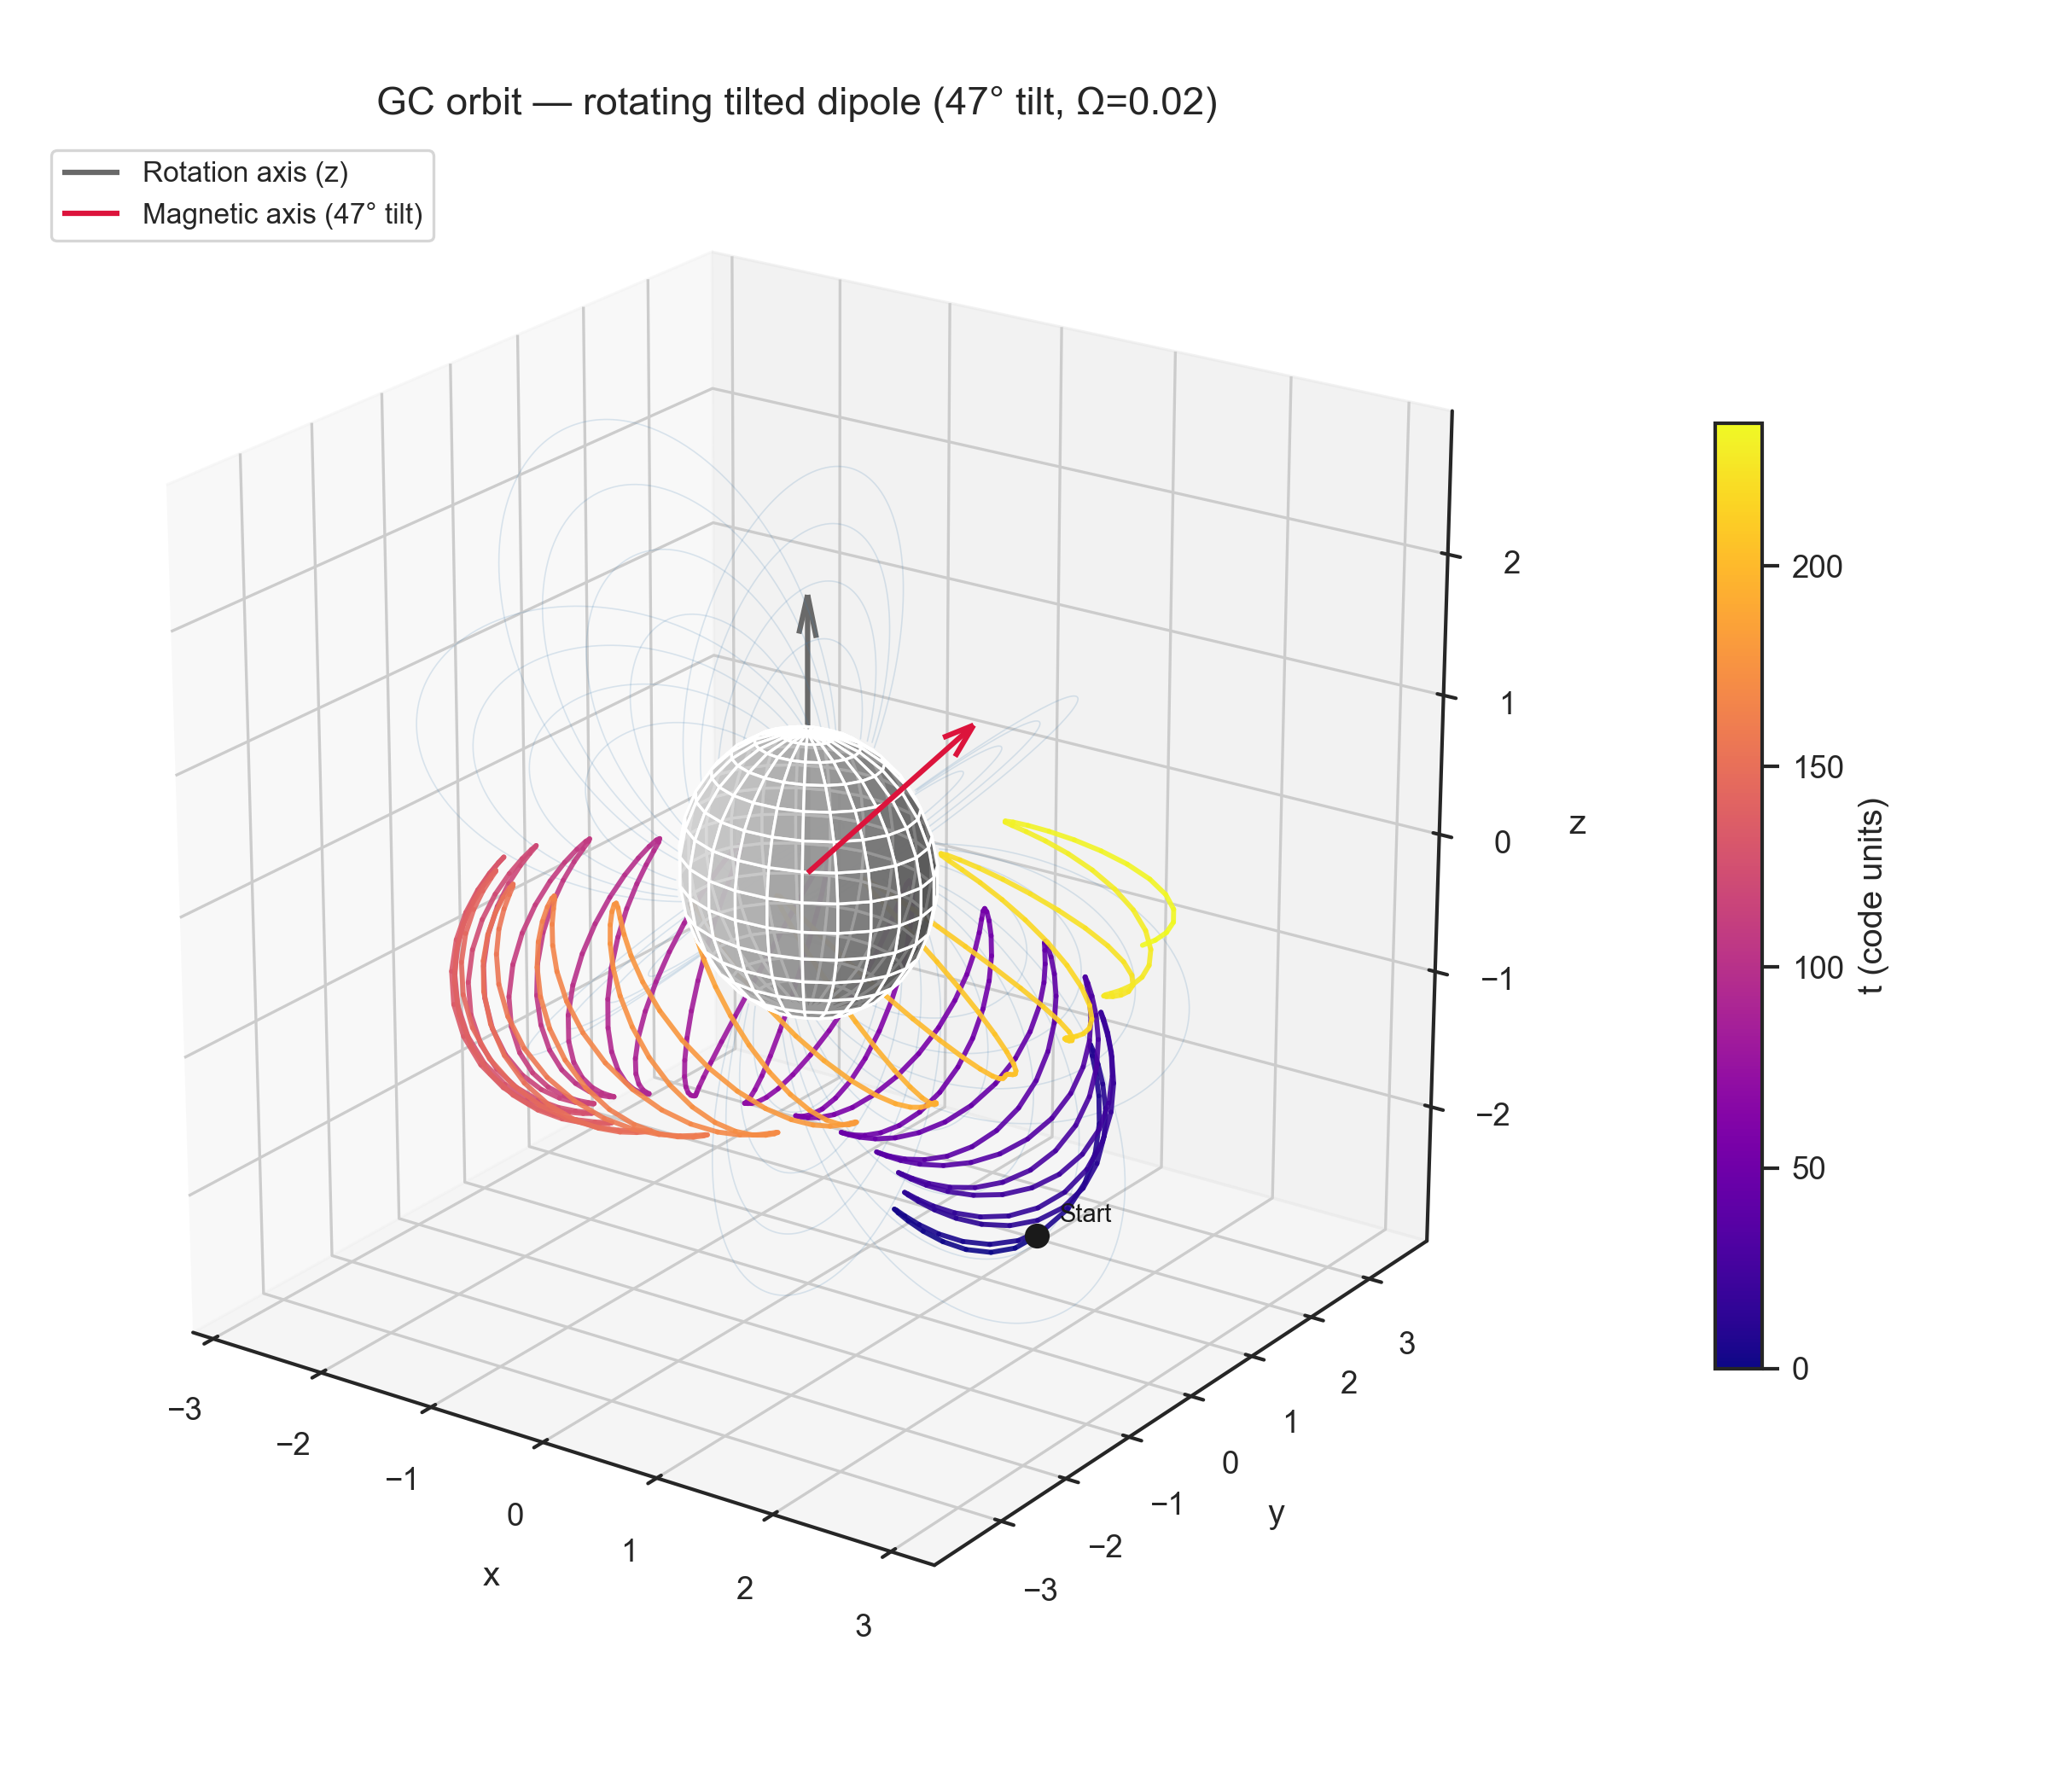
\includegraphics[width=0.55\textwidth]{Figures/test16_rotating_dipole_3D.png}
  \caption{3D guiding-centre orbit in a rotating tilted dipole
    ($47^\circ$ tilt, $\Omega = 0.02$), coloured by time. The magnetic
    axis (red) rotates about the geographic axis (grey). Field lines
    are shown at $t = 0$ for geometric context.}
  \label{fig:rot_3D}
\end{figure}

The total azimuthal drift rate $\Omega_\mathrm{meas} \approx 0.026$
exceeds the input $\Omega = 0.02$, consistent with the additional
gradient and curvature drift contribution measured in
Section~\ref{sec:corotation}.
